% =============================================================================
%  TFM: Trabajo Fin de Máster
%  MU Bioinformática · Universidad Nebrija
%  Compilación (sin citas aún):  pdflatex main.tex && pdflatex main.tex
%  Compilación (con \cite{...}):  pdflatex → bibtex → pdflatex → pdflatex
%  Nota: bibtex falla con "no \citation commands" hasta que haya citas en el texto.
%  En Overleaf:  seleccionar pdfLaTeX como compilador (menú → Settings).
% =============================================================================

\documentclass[12pt,a4paper]{article}

% --- Codificación y tipografía -----------------------------------------------
\usepackage[utf8]{inputenc}
\usepackage[T1]{fontenc}
\usepackage{lmodern}
\usepackage{microtype}
% \usepackage[spanish]{babel} % Opcional: activar si el idioma esta instalado en TinyTeX.

% --- Página ------------------------------------------------------------------
\usepackage{geometry}
\geometry{left=25mm, right=25mm, top=30mm, bottom=30mm}
\usepackage{setspace}\onehalfspacing
% \usepackage[left]{lineno}\linenumbers   % Descomentar para revisión (doble numeración)

% --- Matemáticas -------------------------------------------------------------
\usepackage{amsmath,amssymb}
\usepackage{siunitx}
\sisetup{group-separator={,}}

% --- Figuras y subfiguras ----------------------------------------------------
\usepackage{graphicx}\graphicspath{{../figures/}}
\usepackage[font=small,labelfont=bf,labelsep=period]{caption}
\usepackage{subcaption}

% --- Tablas ------------------------------------------------------------------
\usepackage{booktabs,array,multirow,longtable}
\usepackage{float}
\usepackage{tabularx}
\newcolumntype{Y}{>{\centering\arraybackslash}X}

% --- Listas ------------------------------------------------------------------
\usepackage{enumitem}\setlist{nosep}

% --- Código fuente -----------------------------------------------------------
\usepackage{listings}
\lstset{
  basicstyle       = \small\ttfamily,
  keywordstyle     = \bfseries\color{blue!70!black},
  commentstyle     = \itshape\color{gray},
  stringstyle      = \color{red!60!black},
  numberstyle      = \tiny\color{gray},
  numbers          = left,
  numbersep        = 6pt,
  frame            = single,
  framerule        = 0.4pt,
  rulecolor        = \color{black!30},
  backgroundcolor  = \color{black!3},
  breaklines       = true,
  showstringspaces = false,
  tabsize          = 4,
  captionpos       = b,
  aboveskip        = 10pt,
  belowskip        = 6pt,
}
\lstdefinestyle{python}{language=Python,
  morekeywords={as,with,True,False,None}}
\lstdefinestyle{R}{language=R,
  morekeywords={library,function,if,else,for,in,TRUE,FALSE,NULL}}
\lstdefinestyle{bash}{language=bash,
  morekeywords={snakemake,conda,pip}}

% --- Cajas destacadas (tipo Box de Nature Reviews) ---------------------------
\usepackage{tcolorbox}
\newtcolorbox{infobox}[1][]{
  colback=blue!3, colframe=blue!40!black,
  fonttitle=\bfseries, coltitle=white, colbacktitle=blue!40!black,
  boxrule=0.5pt, arc=2pt, left=6pt, right=6pt, title={#1}}
\newtcolorbox{keypoint}[1][]{
  colback=yellow!5, colframe=orange!60!black,
  fonttitle=\bfseries,
  boxrule=0.4pt, arc=2pt, left=6pt, right=6pt, title={#1}}

% --- TikZ (diagramas) -------------------------------------------------------
\usepackage{tikz}
\usetikzlibrary{shapes.geometric,arrows.meta,positioning,calc}

% --- Hipervínculos -----------------------------------------------------------
\usepackage[colorlinks,
            linkcolor=black,
            citecolor=blue!60!black,
            urlcolor=blue!60!black]{hyperref}
\usepackage[capitalise,noabbrev]{cleveref}

% --- Bibliografía: BibTeX clásico con natbib ---------------------------------
\usepackage[numbers,sort&compress]{natbib}
\bibliographystyle{unsrtnat}
\renewcommand{\bibsection}{\section{Bibliografía}}

% --- Comandos personalizados -------------------------------------------------
\newcommand{\gene}[1]{\textit{#1}}
\newcommand{\tool}[1]{\textsc{\lowercase{#1}}}
\newcommand{\pvalue}{\ensuremath{p}}
\newcommand{\padj}{\ensuremath{p_{\text{adj}}}}
\newcommand{\foldchange}{\ensuremath{\log_2\text{FC}}}
\renewcommand{\abstractname}{Resumen}
\renewcommand{\contentsname}{Índice}
\renewcommand{\listfigurename}{Índice de figuras}
\renewcommand{\listtablename}{Índice de tablas}

% --- Metadatos ---------------------------------------------------------------
\title{Benchmarking de modelos de ML supervisado para predicción de
variables clínicas binarias en R/tidymodels}
\author{Jose Rafael Camacho Custodio%
  \thanks{Máster en Bioinformática, Universidad Nebrija.}}
\date{22 Junio 2026}

% =============================================================================
\begin{document}
\maketitle

% --- Resumen -----------------------------------------------------------------
\begin{abstract}\noindent
La aplicación de modelos de aprendizaje automático (Machine Learning)
supervisado en medicina predictiva
depende no solo de la capacidad de los algoritmos, sino también de la calidad
metodológica con la que se preparan los datos clínicos. En este trabajo se
desarrolla un benchmarking para evaluar el impacto de dos
estrategias de preprocesamiento sobre la predicción de mortalidad hospitalaria
(\textit{hospdead}) en el dataset SUPPORT2, una cohorte multicéntrica de
pacientes críticos con alta heterogeneidad clínica, valores faltantes
informativos y riesgo potencial de fuga de datos (\textit{Data Leakage}). La estrategia V1
(Bio Data) incorpora razonamiento clínico-estadístico mediante imputación
estratificada por diagnóstico, exclusión de variables derivadas o temporales y
tratamiento contextual de la ausencia de datos. La estrategia V2 (Tech Data)
representa un enfoque técnico-estadístico basado en reglas puramente técnicas,
sin considerar la lógica biológica ni el contexto clínico.

Sobre ambas versiones del dataset se entrenaron y evaluaron modelos de
clasificación binaria, incluyendo Logistic Regression, Decision Tree, Random
Forest, XGBoost, Naive Bayes y K-Nearest Neighbors,
mediante una arquitectura reproducible en R/tidymodels. El dataset fue dividido
en entrenamiento, validación y prueba final; la validación cruzada se ejecutó
dentro del conjunto de entrenamiento, mientras que el entrenamiento simple
utilizó el conjunto de validación externo para la selección de configuraciones.
Los resultados muestran que los modelos de ensamble, especialmente Random Forest
y XGBoost, alcanzaron el mejor rendimiento global. Desde una perspectiva
puramente métrica, la estrategia V2 obtuvo los valores más altos de área bajo la
curva ROC (AUC-ROC), cercanos a 0.974 en validación cruzada y 0.979 en
evaluación externa, mientras que V1 mantuvo un rendimiento competitivo, con
valores alrededor de 0.920 en validación y entre 0.927 y 0.932 en evaluación
externa según el esquema experimental. Sin embargo, esta diferencia revela una
tensión metodológica central: el mayor rendimiento numérico puede estar
influido por la retención de variables con menor validez clínica o con riesgo
de introducir información no disponible en un escenario predictivo real. En
conjunto, los hallazgos indican
que la hipótesis inicial se confirma de forma parcial: el preprocesamiento
informado por conocimiento clínico no maximiza necesariamente el AUC bruto,
pero sí contribuye a construir modelos más interpretables, metodológicamente
prudentes y coherentes con la lógica biomédica.
\medskip\noindent
\textbf{Palabras clave:} Machine Learning supervisado, medicina predictiva,
SUPPORT2, mortalidad hospitalaria, preprocesamiento de datos, fuga de datos,
benchmarking, V1, V2, tidymodels
\end{abstract}

% --- Índice ------------------------------------------------------------------
\newpage
\tableofcontents

% --- Índice de tablas y figuras ----------------------------------------------
\newpage
\listoffigures
\newpage
\listoftables

% --- Secciones principales ---------------------------------------------------
\newpage
\section{Introducción}\label{sec:intro}

\subsection{Contexto}

En el ámbito de la medicina predictiva, la efectividad de los modelos de Machine Learning (ML) supervisados no reside únicamente en la sofisticación de sus arquitecturas algorítmicas, sino en la integridad y el tratamiento metodológico de los datos que los alimentan.

Los datasets clínicos y biomédicos presentan desafíos intrínsecos que los
diferencian de otros dominios: altos volúmenes de valores faltantes (missing
values), distribuciones asimétricas, multicolinealidad entre biomarcadores y,
fundamentalmente, el riesgo de Data Leakage. En medicina, un
dato faltante rara vez es un error de registro aleatorio; a menudo, es una señal
clínica o un protocolo hospitalario específico.
Por tanto, el preprocesamiento se convierte en la etapa más
crítica del ciclo de vida del dato, pues una decisión puramente técnica puede
destruir la coherencia biológica necesaria para que un modelo sea útil en un
entorno clínico real.

En la construcción de flujos de trabajo (pipelines) de ciencia de datos, es habitual el empleo de estrategias de preprocesamiento de naturaleza técnica, tales como la imputación basada en tendencias centrales globales (medias o medianas), la eliminación de variables según umbrales estadísticos de nulidad o la selección de características mediante algoritmos de aprendizaje. Si bien estos métodos aseguran la eficiencia computacional, plantean un escenario de interés para la investigación: evaluar el impacto diferencial que aporta la integración del razonamiento clínico-estadístico en la preparación de los datos.

Por lo tanto, esta investigación se centra en la necesidad de establecer un marco comparativo robusto o benchmarking. El objetivo es cuantificar y analizar cómo influye un enfoque de preprocesamiento informado por la lógica médica y el análisis contextual del dataset en el rendimiento, la estabilidad y la fiabilidad de los modelos de aprendizaje automático. De este modo, el estudio busca determinar si esta personalización del pipeline genera diferencias significativas en la capacidad de discriminación diagnóstica frente a las estrategias técnicas estandarizadas aplicadas a variables clínicas binarias.

\subsection{Hipótesis}\label{sec:hipotesis}

Sobre la base del problema expuesto, se plantea la siguiente hipótesis de
investigación:

Las estrategias de preprocesamiento diseñadas mediante el uso de razonamiento
clínico-estadístico y un análisis contextual profundo del dataset generan
resultados predictivos superiores y modelos más robustos en comparación con las
estrategias puramente técnicas o automáticas aplicadas sobre datasets biomédicos
complejos.

Se asume que la integración del conocimiento experto permite identificar
variables informativas ocultas en el ruido y mitigar sesgos metodológicos que
las reglas estadísticas estándar no son capaces de detectar.

\subsection{Objetivos}

\textbf{Objetivo general}

Comparar el impacto de diferentes estrategias de preprocesamiento de datos sobre
el rendimiento de modelos de aprendizaje supervisado aplicados a la predicción
de variables clínicas binarias en un entorno de cuidados críticos.

\textbf{Objetivos específicos}

\begin{itemize}
  \item Diseñar una estrategia clínico-estadística (V1): Construir un flujo de
    procesamiento fundamentado en la lógica médica, utilizando imputaciones
    estratificadas por diagnóstico y una depuración selectiva de variables
    basada en la prevención de Data Leakage y la coherencia biológica.
  \item Diseñar una estrategia técnico-estadística (V2): Desarrollar un flujo de
    procesamiento basado en heurísticas técnicas convencionales y criterios de
    tendencia central global, actuando como grupo de control agnóstico al
    dominio médico.
  \item Construir e implementar un sistema de benchmarking: Desarrollar una
    infraestructura automatizada en R/tidymodels que permita el entrenamiento y
    evaluación sistemática de diversos algoritmos (Random Forest, GBM, Logistic
    Regression, entre otros) sobre las distintas versiones del dataset.
  \item Comparar y evaluar el rendimiento de los modelos: Analizar la capacidad de
    discriminación de los modelos mediante métricas de área bajo la curva
    (AUC-ROC), sensibilidad y especificidad en cada escenario de
    preprocesamiento.
  \item Analizar el impacto del preprocesamiento: Determinar cuantitativa y
    cualitativamente en qué medida el razonamiento clínico influye en la
    estabilidad y precisión de las predicciones frente a las estrategias
    automáticas.
\end{itemize}

\section{Estado del arte y marco teórico}\label{sec:estado-arte}

\subsection{Aprendizaje automático supervisado en salud}

El aprendizaje automático (Machine Learning, ML) ha adquirido una gran relevancia dentro del sector sanitario debido al crecimiento en la disponibilidad de datos clínicos digitales y registros hospitalarios electrónicos~\citep{bajwa2021,davenport2019}. Estas técnicas permiten identificar patrones complejos dentro de grandes volúmenes de información médica, facilitando tareas relacionadas con clasificación, predicción y apoyo a decisiones clínicas.
Dentro de este contexto, el aprendizaje supervisado representa uno de los enfoques más utilizados en aplicaciones médicas~\citep{shamout2021,delpino2025}. Su uso ha permitido desarrollar modelos capaces de predecir distintos desenlaces clínicos a partir de variables fisiológicas, demográficas y hospitalarias. Diversas investigaciones reportan aplicaciones exitosas del ML supervisado en áreas como detección temprana de enfermedades, análisis de imágenes médicas, predicción de riesgo clínico y evaluación de supervivencia de pacientes.

\subsubsection{Modelos supervisados para clasificación binaria}

Los modelos supervisados de clasificación binaria representan una de las técnicas más utilizadas dentro del aprendizaje automático aplicado a problemas médicos y clínicos. Este enfoque consiste en entrenar algoritmos utilizando datos previamente etiquetados con el objetivo de predecir una variable objetivo compuesta por dos posibles clases, como presencia o ausencia de enfermedad, supervivencia o fallecimiento, entre otros escenarios clínicos.
En el ámbito sanitario, los modelos supervisados permiten identificar relaciones entre variables clínicas y desenlaces médicos específicos, facilitando tareas relacionadas con diagnóstico, estratificación de riesgo y apoyo a decisiones clínicas. Debido a esto, múltiples investigaciones han utilizado algoritmos tradicionales de clasificación para evaluar el comportamiento predictivo sobre conjuntos de datos médicos estructurados~\citep{james2021,sklearn_supervised}.

\subsubsection{Modelos tradicionales de clasificación}

Dentro de los modelos supervisados más utilizados en tareas de clasificación binaria se encuentran la regresión logística, los árboles de decisión, Random Forest, Gradient Boosting, K-Nearest Neighbors y Naive Bayes.
La regresión logística es uno de los algoritmos más utilizados en problemas clínicos debido a su simplicidad, interpretabilidad y capacidad para modelar probabilidades asociadas a eventos binarios. Por otro lado, los árboles de decisión permiten representar decisiones mediante estructuras jerárquicas fácilmente interpretables y resultan útiles como línea base en datos estructurados.
Random Forest corresponde a un método de ensamblaje basado en múltiples árboles de decisión, permitiendo mejorar la estabilidad y la capacidad predictiva respecto a modelos individuales. Además, suele comportarse bien en conjuntos de datos clínicos con relaciones no lineales y variables heterogéneas, por lo que constituye una referencia frecuente en benchmarking supervisado.
Gradient Boosting, por su parte, construye secuencialmente árboles débiles para corregir errores previos y suele ofrecer un equilibrio competitivo entre rendimiento y flexibilidad. En problemas médicos tabulares, este tipo de enfoque puede capturar interacciones complejas entre variables sin requerir supuestos paramétricos estrictos.
K-Nearest Neighbors (KNN) clasifica observaciones considerando la cercanía entre instancias dentro del espacio de variables, por lo que puede capturar relaciones locales sin imponer supuestos paramétricos fuertes. Por su parte, Naive Bayes utiliza principios probabilísticos basados en el teorema de Bayes, asumiendo independencia condicional entre variables predictoras. Esta simplicidad lo convierte en una referencia útil como línea base en problemas clínicos con variables mixtas y conjuntos de datos moderados.
En conjunto, estos modelos continúan siendo ampliamente utilizados dentro de investigaciones clínicas y de benchmarking de aprendizaje automático debido a su capacidad de clasificación, facilidad de implementación y adaptabilidad a distintos tipos de conjuntos de datos médicos~\citep{james2021}.

\subsection{Evaluación experimental y benchmarking}

La evaluación experimental constituye una etapa fundamental dentro del desarrollo de modelos de aprendizaje automático, especialmente en aplicaciones clínicas donde la confiabilidad y capacidad de generalización de los modelos resultan críticas. En este contexto, el benchmarking permite comparar distintos algoritmos supervisados bajo condiciones experimentales controladas, utilizando métricas estandarizadas y estrategias consistentes de validación.
El benchmarking tiene como objetivo analizar el comportamiento relativo de múltiples modelos frente a un mismo problema, permitiendo identificar diferencias en rendimiento, estabilidad y capacidad predictiva~\citep{delpino2025}. Dentro del ámbito sanitario, este enfoque resulta particularmente relevante debido a la complejidad de los conjuntos de datos clínicos y a la necesidad de obtener resultados reproducibles y clínicamente confiables.

\subsubsection{Benchmarking de modelos supervisados}

El benchmarking de modelos supervisados consiste en la comparación sistemática de distintos algoritmos de clasificación utilizando un mismo conjunto de datos y condiciones experimentales similares. Este enfoque permite evaluar fortalezas y limitaciones de cada modelo respecto a un problema específico.
Diversas investigaciones destacan la importancia de mantener estrategias consistentes de partición de datos, preprocesamiento y validación experimental durante el benchmarking, ya que pequeñas variaciones metodológicas pueden afectar considerablemente los resultados obtenidos~\citep{delpino2025,moassefi2023}. En aplicaciones médicas, esto adquiere especial relevancia debido a la sensibilidad de los datos clínicos y al impacto potencial de los modelos sobre decisiones sanitarias.

\subsubsection{Métricas de clasificación}\label{sec:metricas-clasificacion}

La evaluación de modelos supervisados requiere métricas capaces de medir diferentes aspectos del desempeño predictivo. Entre las métricas más utilizadas se encuentran Accuracy, Precision, Recall, F1-score y ROC-AUC.
Accuracy representa la proporción total de predicciones correctas realizadas por el modelo respecto al total de observaciones evaluadas. Precision mide la proporción de predicciones positivas correctas respecto al total de positivos predichos por el modelo.
Recall, también conocido como sensibilidad, evalúa la capacidad del modelo para identificar correctamente los casos positivos reales. Por su parte, el F1-score corresponde a la media armónica entre Precision y Recall, permitiendo obtener una medida balanceada del desempeño del modelo.
Finalmente, ROC-AUC mide la capacidad discriminativa del modelo considerando diferentes umbrales de clasificación, siendo ampliamente utilizada en investigaciones médicas debido a su capacidad para evaluar el comportamiento global de modelos binarios~\citep{owusuadjei2023}.

En problemas clínicos de clasificación binaria, la selección de métricas debe
considerar tanto la discriminación global como los errores específicos de cada
clase. Por ello, ROC-AUC resulta útil para comparar la capacidad discriminativa
general de los modelos, mientras que sensibilidad y especificidad permiten
evaluar de forma separada la identificación de pacientes fallecidos y
supervivientes. Accuracy puede utilizarse como métrica complementaria, aunque su
interpretación debe realizarse con cautela cuando existe desbalance de clases.

\subsubsection{Validación experimental y reproducibilidad}

La validación experimental busca garantizar que el rendimiento observado durante el entrenamiento pueda mantenerse sobre datos no utilizados previamente. Para ello, es común dividir los datos en conjuntos de entrenamiento y validación, permitiendo evaluar la capacidad de generalización de los modelos.
La reproducibilidad constituye además un aspecto fundamental dentro de investigaciones basadas en aprendizaje automático aplicado a la salud. La literatura científica señala que múltiples estudios presentan dificultades de reproducibilidad debido a configuraciones experimentales insuficientemente documentadas, diferencias en preprocesamiento o falta de acceso a datos y código fuente~\citep{moassefi2023}.

\subsection{Trabajos relacionados}

\subsubsection{Predicción de riesgo de insuficiencia cardíaca mediante benchmarking supervisado}

Un estudio reciente orientado a la predicción de riesgo de insuficiencia cardíaca desarrolló un benchmarking sistemático de diez algoritmos supervisados utilizando un dataset compuesto por 2,169 pacientes y 15 variables clínicas~\citep{li2026}. Los autores evaluaron modelos tradicionales como Logistic Regression, Decision Trees, Gradient Boosting, K-Nearest Neighbors y Naive Bayes, además de modelos ensemble como Random Forest, XGBoost, LightGBM y CatBoost.
El experimento fue realizado bajo condiciones metodológicas controladas, utilizando el mismo preprocesamiento, partición estratificada de entrenamiento/prueba y métricas estandarizadas de evaluación como ROC-AUC, Accuracy, Precision, Recall y F1-score. Los resultados mostraron que la regresión logística obtuvo el mejor desempeño global, alcanzando un ROC-AUC de 0.9451 y superando modelos más complejos basados en ensamblajes.
El estudio concluye que modelos tradicionales e interpretables pueden mantener un alto rendimiento predictivo sobre datasets clínicos moderados, resaltando además la importancia del benchmarking bajo condiciones reproducibles y consistentes para realizar comparaciones válidas entre algoritmos supervisados.

\subsubsection{Framework RISA para clasificación clínica e interpretabilidad}

Otro trabajo relevante propuso el framework RISA (Robust and Interpretable Simulation-Analysis), orientado a evaluar robustez, interpretabilidad y capacidad de generalización de modelos supervisados aplicados al diagnóstico de apendicitis aguda~\citep{uddin2026}.
El estudio evaluó seis algoritmos supervisados mediante 24 escenarios factoriales que incorporaban factores como desbalance de clases, dimensionalidad, heterogeneidad y fronteras de decisión no lineales. Posteriormente, los modelos fueron validados utilizando dos datasets clínicos independientes relacionados con pacientes adultos y pediátricos.
Los resultados mostraron diferencias significativas en el comportamiento de los modelos dependiendo de la complejidad estructural del dataset y las características estadísticas presentes en cada escenario experimental. Además, el estudio incorporó técnicas de interpretabilidad mediante SHAP y LIME para validar la relevancia clínica de las variables utilizadas por los modelos.
Los autores destacan que estrategias reproducibles y transparentes de benchmarking permiten construir modelos clínicos más robustos y confiables para aplicaciones reales en salud.

\subsubsection{Predicción de mortalidad en UCI mediante Machine Learning}

En otra investigación reciente, se desarrolló un modelo predictivo para mortalidad a 28 días en pacientes con pancreatitis aguda ingresados en unidades de cuidados intensivos~\citep{wei2026}. El estudio utilizó datos clínicos obtenidos de las bases MIMIC-IV y eICU-CRD, incorporando biomarcadores derivados como LAR, BAR y RAR junto con variables clínicas tradicionales.
Los autores aplicaron técnicas de selección de variables utilizando el algoritmo Boruta y desarrollaron siete modelos supervisados de Machine Learning para comparar rendimiento predictivo. El benchmarking fue complementado mediante validación cruzada interna y validación externa sobre un segundo dataset independiente.
Dentro de los modelos evaluados, ExtraTrees obtuvo el mejor desempeño general, alcanzando un AUC de 0.8546 durante entrenamiento y 0.82 en validación externa. El estudio resalta además la importancia de combinar selección de variables, benchmarking supervisado y validación externa para mejorar la capacidad de generalización de modelos clínicos.

\section{Metodología}\label{sec:metodologia}

\subsection{Enfoque metodológico}

El diseño metodológico del presente trabajo se basa en la construcción de un benchmarking sistemático para determinar cómo las decisiones en la etapa de preparación de datos condicionan el rendimiento de modelos de aprendizaje supervisado en el dominio clínico.

\subsection{Evaluación y selección de datasets}

\textbf{Objetivo de la evaluación inicial}

La fase inicial de selección de datos constituyó una etapa crítica en la
configuración metodológica. El objetivo primordial no fue simplemente adquirir un conjunto de datos biomédicos, sino identificar un entorno de información que presentara una complejidad intrínseca y desafíos en el preprocesamiento, adecuados para validar la hipótesis central
del estudio (Sección~\ref{sec:hipotesis}). Para ello, se requería un conjunto de datos que reflejara la heterogeneidad y los desafíos de los datos reales en salud, incluyendo valores faltantes, informativos, multicolinealidad fisiológica y el potencial de fuga de datos
temporal o estructural.

\textbf{Datasets evaluados y desestimados}

Breast Cancer Wisconsin (Diagnostic)~\citep{wolberg1993}

\begin{itemize}
  \item Descripción breve: Este dataset, ampliamente utilizado en la comunidad de
    Machine Learning, se centra en la clasificación de tumores mamarios como
    benignos o malignos. Contiene 569 observaciones y 32 variables, la mayoría
    de las cuales son medidas biomédicas numéricas continuas (e.g., radius\_mean,
    texture\_mean, perimeter\_mean) derivadas de imágenes digitalizadas de masas
    celulares. La variable objetivo es el diagnóstico clínico (M para maligno, B
    para benigno).
  \item Ventajas observadas: Es un dataset excepcionalmente "limpio", con una
    documentación exhaustiva y es un referente estándar para el benchmarking de
    algoritmos de clasificación. La ausencia de valores nulos significativos
    simplifica su uso.
  \item Limitaciones observadas: A pesar de sus ventajas, su baja complejidad
    clínica y estructural lo hizo inadecuado para los objetivos de este
    estudio. La escasez de valores faltantes (no se observaron valores nulos en
    ninguna de las 569 observaciones) limita drásticamente la oportunidad de
    explorar estrategias avanzadas de imputación basadas en conocimiento
    clínico. Además, al consistir principalmente en variables numéricas ya
    procesadas, ofrece un espacio reducido para el análisis profundo de la
    heterogeneidad de variables categóricas, económicas o de gestión
    hospitalaria, desviándose de la intención de demostrar la robustez del
    preprocesamiento en escenarios más realistas.
\end{itemize}

Parkinsons~\citep{little2007}

\begin{itemize}
  \item Descripción breve: Se evaluó el dataset parkinsons.data, el cual contiene
    195 observaciones y 24 variables biomédicas derivadas de señales de voz,
    destinadas a clasificar la presencia de la enfermedad de Parkinson. La
    variable objetivo es status (0 para sanos, 1 para pacientes).
  \item Ventajas observadas: Representa un problema clínico relevante y utiliza
    señales biomédicas reales.
  \item Limitaciones observadas: Su principal limitación para este estudio fue su
    tamaño extremadamente reducido. Con tan solo 195 registros, la capacidad de
    generalización y la robustez de los modelos entrenados se verían
    comprometidas, especialmente en un contexto de benchmarking con múltiples
    estrategias. Además, presenta una menor heterogeneidad de variables en
    comparación con un entorno hospitalario complejo, lo que reduce el alcance
    para explorar estrategias avanzadas de imputación o selección de variables
    que trasciendan lo puramente estadístico. La relativa "perfección" de sus
    datos y la menor riqueza clínica y hospitalaria también lo desvían del
    propósito de este TFM.
\end{itemize}

Chronic Kidney Disease (CKD)~\citep{rubini2015}

\begin{itemize}
  \item Descripción breve: Este dataset busca clasificar la presencia de enfermedad
    renal crónica (ckd o notckd) en pacientes, a partir de 400 observaciones
    y 25 variables clínicas y biomédicas, que incluyen parámetros fisiológicos,
    análisis sanguíneos y condiciones clínicas del paciente.
  \item Ventajas observadas: Representa un problema clínico relevante y exhibe una
    mezcla de variables numéricas y categóricas, junto con una cantidad
    considerable de valores faltantes en múltiples variables (ej., rbc, rbcc,
    wbcc, pot).
  \item Limitaciones observadas: A pesar de ser más prometedor en términos de
    presencia de NAs y diversidad de variables, su tamaño limitado (400
    observaciones) y su menor diversidad clínica en comparación con escenarios
    hospitalarios de cuidados críticos lo hicieron menos adecuado. La escala del
    dataset no permitía una exploración tan exhaustiva de la interacción entre
    variables complejas o la validación de estrategias de preprocesamiento
    avanzadas con la solidez requerida para un estudio de benchmarking integral.
\end{itemize}

\textbf{Criterios de evaluación y razones de la desestimación}

Los datasets evaluados, si bien válidos para propósitos académicos específicos,
fueron finalmente descartados por presentar limitaciones críticas para los
objetivos de este trabajo. Los criterios de evaluación considerados fueron:

\begin{itemize}
  \item Complejidad Clínica y Estructural: La capacidad del dataset para reflejar la
    interconexión de múltiples factores clínicos, demográficos y
    administrativos.
  \item Diversidad de Variables: La presencia de una mezcla amplia de variables
    continuas, categóricas, demográficas y administrativas.
  \item Tamaño del Dataset: Un número suficiente de registros para asegurar la
    robustez estadística de los modelos y la estabilidad de las particiones.
\end{itemize}

Estos factores reducirían la capacidad de demostrar el
impacto diferencial de un preprocesamiento avanzado y la comprensión de las
decisiones tomadas bajo un razonamiento clínico-estadístico.

\subsection{Selección del dataset SUPPORT2}

\textbf{Justificación de selección y variable objetivo}

El dataset SUPPORT2 (Study to Understand Prognoses and Preferences for Outcomes
and Risks of Treatments)~\citep{knaus_support2} fue seleccionado como el eje central de este estudio
por su alta dimensionalidad, riqueza de información y su fiel representación
de los desafíos inherentes a los datos hospitalarios del mundo real. Este
dataset no solo ofrece una alta dimensionalidad con 9,105 registros y 47
variables, sino que también presenta patrones de datos faltantes significativos
y una profunda interconexión de variables que demandan un análisis exploratorio
y un preprocesamiento rigurosos.

\textbf{Justificación de la Variable Objetivo: hospdead}

La variable hospdead (mortalidad hospitalaria) fue elegida como la variable
objetivo principal para el problema de clasificación binaria. Esta decisión se
fundamenta en un análisis detallado que considera la naturaleza del
dataset, su contexto clínico original y las observaciones clave del EDA:

\begin{enumerate}
  \item Coherencia con el Diseño del Dataset: La documentación original de SUPPORT2
    y su propósito principal se centran en la predicción del pronóstico y los
    outcomes en pacientes críticos. hospdead representa un desenlace directo y
    central a esta misión, caracterizando un evento bien definido dentro del
    período de hospitalización.
  \item Relevancia Clínica y Metodológica: La mortalidad intrahospitalaria es una
    métrica de alto interés biomédico, fundamental para la predicción de riesgo, la toma de decisiones clínicas y la evaluación de
    la severidad del paciente. Al integrar múltiples variables
    fisiológicas, funcionales y clínicas agudas, está especialmente diseñado
    para modelar la evolución del paciente durante la hospitalización, haciendo
    de hospdead un outcome natural y congruente.
  \item Estabilidad frente a Alternativas:
    \begin{itemize}
      \item death (mortalidad general): Aunque también representa mortalidad, death
        abarca un horizonte temporal más amplio (hasta seis meses post-ingreso,
        incluyendo eventos fuera del hospital) y puede incorporar mayor pérdida
        de seguimiento y factores externos. hospdead ofrece una variable
        objetivo más controlada y estable para un problema de clasificación
        supervisada.
      \item Variables Diagnósticas (dzgroup, dzclass): Transformar estas variables
        categóricas complejas en un problema binario (ej., "cáncer vs. no
        cáncer") implicaría agrupar condiciones clínicas dispares bajo una
        clase negativa, lo que reduciría la coherencia biológica y la
        discriminación inherente al dataset.
      \item Condiciones Crónicas (diabetes, dementia): Estas variables, si bien
        importantes, se relacionan más con características preexistentes del
        paciente que con la evolución clínica aguda en el hospital, que es el
        foco principal de SUPPORT2 y de muchas de sus variables fisiológicas.
    \end{itemize}
\end{enumerate}

Durante el EDA, se observaron patrones de relación intrigantes entre hospdead y
una amplia gama de predictores (histogramas, boxplots, correlaciones). Estos
patrones sugirieron que hospdead es una variable rica en información, capaz de
revelar cómo las interacciones complejas de factores clínicos y administrativos
influyen en el pronóstico, lo que la convierte en una elección óptima para
construir un modelo predictivo robusto.

\textbf{Descripción general del dataset}

El dataset SUPPORT2 es el resultado de un estudio multicéntrico observacional
que recopiló información clínica detallada de 9,105 pacientes adultos ingresados
en cinco hospitales de Estados Unidos entre 1989 y 1994. Estos pacientes
padecían enfermedades graves en fase avanzada, incluyendo insuficiencia
respiratoria aguda, EPOC, insuficiencia cardíaca congestiva, cirrosis, cáncer,
coma y fallo multiorgánico. El objetivo principal del estudio fue analizar el
pronóstico, la evolución clínica y los outcomes hospitalarios, especialmente la
mortalidad y las preferencias de atención al final de la vida. La magnitud y
profundidad de los datos recopilados lo establecen como un recurso de referencia
en la investigación de outcomes en pacientes críticos.

\textbf{Tipos de variables presentes}

La riqueza del dataset radica en su diversidad de 47 variables, que abarcan
múltiples dominios. El diccionario completo de variables se presenta en el
Anexo~\ref{sec:anexo-diccionario}.

\begin{itemize}
  \item Variables Demográficas: Edad (age), sexo (sex), etnia (race), nivel de
    ingresos (income) y nivel educativo (edu).
  \item Variables Fisiológicas y Analíticas: Constantes vitales como la presión
    arterial media (meanbp), frecuencia cardíaca (hrt), frecuencia respiratoria
    (resp) y temperatura (temp). También incluye marcadores de laboratorio como
    la albúmina sérica (alb), bilirrubina (bili), creatinina (crea), glucosa
    (glucose) y pH sanguíneo (ph).
  \item Scores Clínicos Validados: Índices de severidad como el APACHE III (aps), el
    TISS (avtisst), la puntuación de coma basada en la escala de Glasgow
    (scoma), y la puntuación de fisiología SUPPORT (sps).
  \item Variables de Gestión y Económicas: Días de estancia hospitalaria (slos),
    cargos facturados por el hospital (charges) y costos totales calculados
    (totcst, totmcst).
  \item Variables Funcionales: Índices de Actividades de la Vida Diaria (ADL)
    reportados por el paciente (adlp) y por un familiar (adls).
  \item Variables Derivadas y de Pronóstico: Estimaciones de probabilidad de
    supervivencia a 2 (surv2m, prg2m) y 6 meses (surv6m, prg6m).
\end{itemize}

\subsection{Análisis Exploratorio de Datos (EDA)}

El análisis exploratorio reveló una imagen detallada de la estructura y
características del dataset, identificando patrones cruciales para las
etapas posteriores.

\textbf{Análisis de valores faltantes (Missing Values)}

La integridad de los datos en SUPPORT2 es un aspecto central, con una
distribución de valores nulos que varía desde el 0\% hasta un
considerable 61.9\%. Este patrón de missingness no es aleatorio, sino que es
altamente informativo:

\begin{itemize}
  \item Variables con Alta Ausencia de Datos (Missingness > 40\%):
    \begin{itemize}
      \item adlp (Actividades de la vida diaria previas): 61.95\% de valores
        faltantes (5,641 registros). Crucialmente, los pacientes fallecidos en
        el hospital presentaron un 92\% de nulos en esta variable, frente al 52\%
        de los supervivientes. Esto subraya que la ausencia del dato está
        directamente vinculada con la gravedad extrema del paciente (coma,
        sedación, imposibilidad de responder), y es una señal clínica relevante.
      \item urine (Producción urinaria): 53.40\% de valores faltantes (4,862
        registros).
      \item glucose (Glucosa sérica): 49.42\% de valores faltantes (4,500 registros).
      \item bun (Nitrógeno ureico en sangre): 47.80\% de valores faltantes (4,352
        registros).
    \end{itemize}
  \item Variables con Moderada Ausencia de Datos (Missingness 5\% - 40\%):
    \begin{itemize}
      \item alb (Albúmina sérica): 37.03\% (3,372 registros).
      \item bili (Bilirrubina sérica): 28.57\% (2,601 registros).
      \item pafi (Índice de oxigenación Kirby): 25.54\% (2,325 registros). Se observó
        una menor ausencia en pacientes con patologías respiratorias (ej.,
        un 13.7\% en COPD), sugiriendo una recolección condicionada al protocolo
        clínico.
      \item ph (pH sanguíneo): 25.09\% (2,284 registros). Similar a pafi, con menor
        ausencia en pacientes críticos/respiratorios.
      \item income (Nivel de ingresos): 32.75\%.
      \item adls (Actividades de la vida diaria al seguimiento): 31.49\%. A
        diferencia de adlp, sus patrones de missingness son menos influenciados
        por la gravedad extrema.
    \end{itemize}
  \item Variables con Mínima Ausencia de Datos (Missingness < 5\%):
    \begin{itemize}
      \item Variables vitales como sod (0.01\%), temp (0.01\%), resp (0.01\%), hrt
        (0.01\%), meanbp (0.01\%), surv6m (0.01\%), surv2m (0.01\%), aps (0.01\%),
        sps (0.01\%), scoma (0.01\%). Estas variables, con datos casi completos,
        constituyen el bloque más fiable del dataset.
    \end{itemize}
\end{itemize}

\textbf{Estadísticas descriptivas y distribuciones de variables}

El análisis de las distribuciones y estadísticas descriptivas reveló una
heterogeneidad considerable:

\begin{itemize}
  \item Sesgo Positivo: Una gran mayoría de variables continuas, incluyendo
    crea, bun, bili, wblc, charges, totcst, totmcst, slos (estancia
    hospitalaria) y hday (día de ingreso), muestran una fuerte asimetría
    positiva. Esto se manifiesta con una acumulación de registros en los valores
    bajos y una cola muy larga hacia la derecha. Por ejemplo, slos tiene una
    mediana de 11 días pero un máximo de 343 días, y charges oscila desde una
    mediana de 25,024 hasta un máximo de 1,435,423. Esto refleja una
    población con un estado relativamente estable, pero con un subgrupo de
    casos extremos que disparan los costos y la duración de la estancia.
  \item Comportamientos Bimodales: Variables como la frecuencia cardíaca (hrt),
    presión arterial media (meanbp) y temperatura (temp) exhiben dos picos
    distintos. Esto indica la presencia de dos subpoblaciones claras: pacientes
    con valores dentro de rangos fisiológicos normales y pacientes
    descompensados (ej., taquicardia/bradicardia, hipotensión/hipertensión,
    fiebre/hipotermia).
  \item Comportamientos Multimodales: Las variables de estimación subjetiva del
    pronóstico (prg2m, prg6m) muestran picos espaciados uniformemente
    (25\%, 50\%, 75\%). Este patrón sugiere un sesgo de redondeo por parte de los
    médicos al asignar probabilidades, lo que difiere de una variable biológica
    continua.
  \item Distribución Simétrica/Normal: Variables como la edad (age), el score de
    fisiología SUPPORT (sps), el pH sanguíneo (ph) y la concentración de sodio
    (sod) tienden a una distribución más simétrica o aproximadamente normal.
  \item Variable Objetivo (hospdead): Se observó un desbalance moderado, con 6,745
    pacientes (74.1\%) que sobrevivieron y 2,360 (25.9\%) que fallecieron durante
    la hospitalización.
\end{itemize}

\textbf{Análisis de correlación y detección de fuga de datos}

La matriz de correlación reveló importantes relaciones lineales y potenciales
fuentes de fuga de datos:

\begin{itemize}
  \item Redundancia Alta: Se identificó una correlación perfecta (r = 1.0) entre
    adlsc y adls, indicando que representan la misma información o
    transformaciones idénticas. Similarmente, charges, totcst y totmcst muestran
    correlaciones muy elevadas (superiores a 0.86), apuntando a una fuerte
    redundancia en la información económica.
  \item Leakage Temporal: El tiempo total de seguimiento del paciente (d.time)
    exhibe una marcada correlación inversa de -0.79 con death. Esta fuerte
    relación se debe a que el d.time se trunca abruptamente cuando ocurre el
    fallecimiento, lo que lo convierte en una variable que incorpora información
    del futuro respecto a una predicción al ingreso.
  \item Relación de Variables Derivadas: Las probabilidades estimadas de
    supervivencia a corto y mediano plazo (surv2m, surv6m) se encuentran
    fuertemente vinculadas de manera negativa con el score de severidad
    fisiológica (sps), alcanzando correlaciones de hasta -0.72. Esto sugiere
    que estas variables son, en parte, el resultado de modelos predictivos y no
    mediciones directas.
  \item Consistencia Fisiológica: Biomarcadores de función renal como el nitrógeno
    ureico (bun) y la creatinina (crea) exhiben una correlación positiva
    moderada-alta de 0.66, confirmando una progresión conjunta ante el deterioro
    del sistema urinario.
\end{itemize}

\subsection{Construcción de estrategias de preprocesamiento}

Esta sección detalla las dos aproximaciones metodológicas diseñadas para el
preprocesamiento del dataset SUPPORT2. La comparación de estas estrategias
constituye el núcleo del experimento, permitiendo evaluar si la integración del
conocimiento de dominio mejora la capacidad predictiva y la robustez de los
modelos de aprendizaje automático frente a un enfoque puramente algorítmico.

\subsubsection{Estrategia clínico-estadística (V1)}

\textbf{Filosofía y Razonamiento de Dominio}

La estrategia V1 se diseñó bajo un enfoque de supervisión experta en el proceso
de preprocesamiento. El razonamiento central es que, en un entorno hospitalario,
la ausencia de una medición o la correlación entre variables puede responder a
una lógica clínica, administrativa o temporal. Por lo tanto, la preparación de
los datos debe respetar la coherencia biológica. En lugar de aplicar reglas de
corte genéricas, como eliminar variables por un porcentaje fijo de nulos, se
analizó el origen de cada variable y el motivo de su ausencia para decidir su
permanencia o su forma de imputación.

\textbf{Gestión de la Integridad y Calidad del Dato}

Una premisa clave de esta estrategia es priorizar un conjunto de predictores
clínicamente consistente frente a la retención indiscriminada de variables con
alta incertidumbre o riesgo metodológico.

\begin{itemize}
  \item Eliminación de registros por inconsistencia basal: Se decidió eliminar las
    observaciones incompletas en variables como crea, meanbp, hrt, resp, temp,
    sod, scoma, aps y crea. Al presentar un porcentaje de nulos mínimo (<1.2\%),
    su eliminación supone una pérdida insignificante de registros pero garantiza
    que el modelo solo aprenda de pacientes con un perfil clínico basal
    completo. Además, se comprobó que estos nulos se concentraban en la clase
    mayoritaria, por lo que no se afectó el desbalance del dataset.
  \item Exclusión de variables por baja fiabilidad: Variables como bun y glucose
    fueron eliminadas debido a que sus altísimos niveles de nulos (cercanos
    al 50\%) obligarían a realizar imputaciones masivas que homogeneizarían
    artificialmente la muestra, destruyendo el sentido biológico del dato.
\end{itemize}

\textbf{Prevención de fuga de datos}

\begin{itemize}
  \item Leakage de Modelos Previos: Las variables surv2m y surv6m fueron eliminadas
    por ser estimaciones generadas por otros modelos predictivos, lo que
    inflaría la precisión de forma artificial. Asimismo, basándose en el
    protocolo original de SUPPORT (JAMA, 1995), se identificó que prg2m y prg6m
    formaron parte de una intervención clínica posterior, lo que las inhabilita
    como predictores de línea base.
  \item Fuga temporal: Se eliminó d.time (tiempo de seguimiento) y slos (estancia hospitalaria) por su
    separación matemática perfecta con el desenlace hospdead, y se descartaron
    sps y avtisst por representar métricas procesadas que pueden verse alteradas
    por decisiones terapéuticas posteriores al ingreso.
\end{itemize}

\textbf{Imputación Basada en Contexto y Estratificación}

En lugar de una mediana global, se aplicó una imputación estratificada por
diagnóstico (dzgroup), bajo la lógica de que los valores normales varían según
la patología:

\begin{itemize}
  \item Variables Fisiológicas Condicionadas: Para bili, alb, ph, pafi y wblc, se
    utilizó la mediana del grupo diagnóstico. Es fisiológicamente coherente que
    un paciente con cirrosis tenga una mediana de bilirrubina distinta a uno con
    insuficiencia cardíaca.
  \item Análisis del Blanco Analítico: En el caso de wblc (glóbulos blancos), se
    validó que su ausencia no dependía de estancias cortas (la mediana de
    estancia para estos nulos fue de 9 días), lo que justifica una imputación
    por contexto en lugar de una eliminación.
  \item Incertidumbre Administrativa: Para race, dnr, dnrday y edu, se imputó la
    categoría "Unknown". Se asume que la falta de registro en estas variables
    puede reflejar aspectos administrativos o del proceso de recolección que
    tienen valor predictivo latente.
\end{itemize}

\textbf{Interpretación de la Ausencia Informativa (ADL)}

Uno de los puntos más críticos fue el tratamiento de las escalas funcionales:

\begin{itemize}
  \item Información Oculta en Nulos: En la variable adls, se sustituyeron los nulos
    por la categoría 8 ("No completado"). Se interpreta que el hecho de no poder
    completar el formulario está relacionado con la gravedad o el estado de
    conciencia del paciente.
  \item Exclusión de adlp por Sesgo de Recolección: Se observó que el 92\% de los
    fallecidos no tenían datos en adlp frente al 52\% de los vivos. Aunque tenía
    un alto poder predictivo, se determinó que este poder era un "artefacto" del
    proceso de recolección (los pacientes más graves no podían responder) y no
    una característica fisiológica. Para priorizar la interpretabilidad clínica,
    se decidió eliminarla.
\end{itemize}

\textbf{Refinamiento Estructural}

\begin{itemize}
  \item Eliminación por Redundancia y Control Metodológico: Se eliminó dzclass por
    ser una agrupación redundante de dzgroup, y adlsc por ser una versión ya
    imputada previamente en el estudio original sobre la cual se perdió el
    control metodológico.
  \item Simplificación Económica: Se eliminaron charges (con solo un 2\% de
    nulos), totcst, totmcst e income por su alta correlación y
    baja relevancia clínica directa frente a la mortalidad aguda, además de que
    son variables que no están disponibles al ingreso y pueden introducir fuga
    de datos temporal.
\end{itemize}

Este conjunto de decisiones asegura que V1 no solo sea
estadísticamente apto, sino clínicamente veraz, sentando las bases para un
benchmark donde el conocimiento de dominio sea el factor diferencial.

\begingroup
\footnotesize
\setlength{\tabcolsep}{3pt}
\begin{longtable}{@{}p{0.23\textwidth}p{0.17\textwidth}p{0.21\textwidth}p{0.31\textwidth}@{}}
\caption[Preprocesamiento V1]{Preprocesamiento clínico-estadístico (V1)}\label{tab:preproc-v1}\\
\toprule
\textbf{Variable} & \textbf{Acción} & \textbf{Estrategia aplicada} & \textbf{Observación / Justificación} \\
\midrule
\endfirsthead
\multicolumn{4}{c}{\tablename\ \thetable\ — V1 (continuación)} \\
\toprule
\textbf{Variable} & \textbf{Acción} & \textbf{Estrategia aplicada} & \textbf{Observación / Justificación} \\
\midrule
\endhead
\bottomrule
\endfoot
meanbp, hrt, resp, temp, sod, scoma, aps, crea & Eliminar observaciones & Eliminación puntual & Nulos mínimos en variables basales; se priorizó conservar registros clínicamente completos. \\
race, dnr, edu & Imputar & Categoría ``Unknown'' & La ausencia se trató como información administrativa potencialmente útil. \\
wblc, bili, alb, ph, pafi & Imputar & Mediana por dzgroup & Imputación condicionada por diagnóstico para preservar coherencia fisiológica. \\
adls & Imputar & Valor 8 & Se codificó como ``No completado'', interpretando la ausencia como señal clínica. \\
urine, bun, glucose & Eliminar variable & Missing elevado & La imputación masiva podía homogeneizar artificialmente variables clínicas relevantes. \\
prg2m, prg6m, surv2m, surv6m & Eliminar variable & Riesgo de leakage & Variables pronósticas o derivadas de modelos previos, no adecuadas como predictores basales. \\
death, d.time & Eliminar variable & Leakage directo y temporal & Incorporan información del desenlace o del seguimiento posterior. \\
slos, charges & Eliminar variable & Información posterior & Estancia hospitalaria y cargos acumulados dependen de la evolución clínica y no estarían disponibles al ingreso. \\
totcst, totmcst, income, sfdm2 & Eliminar variable & Missing/redundancia & Baja utilidad clínica directa o alta proporción de ausencia. \\
dnrday, dzclass, adlsc & Eliminar variable & Redundancia y derivación & Información duplicada o ya procesada en variables relacionadas. \\
adlp & Eliminar variable & Sesgo de recolección & Alto poder predictivo asociado al patrón de ausencia, no a una medición fisiológica estable. \\
sps, avtisst & Eliminar variable & Score derivado y leakage & Métricas procesadas o influenciadas por decisiones clínicas posteriores. \\
\end{longtable}
\endgroup

\subsubsection{Estrategia técnico-estadística (V2)}

\textbf{Filosofía y reglas técnico-estadísticas}

Esta aproximación sigue un enfoque técnico-estadístico menos dependiente del
contexto clínico. Las decisiones de preprocesamiento se basan en criterios
generales de partición, completitud de datos y medidas de tendencia central,
sin incorporar razonamiento fisiológico específico para cada variable. Por ello,
funciona como contraste metodológico frente a V1: reproduce decisiones comunes
en flujos computacionales, pero con un componente más arbitrario y menos
informado por el significado biomédico de las variables.

\textbf{Criterios de Selección y Umbrales}

\begin{itemize}
  \item Regla del 35\% de Ausencia: Bajo este enfoque, se establece un umbral
    estricto: cualquier variable con más de un 35\% de valores faltantes es
    eliminada del estudio (alb, bun, glucose, urine, adlp,
    totmcst). Se asume que el ruido introducido por la imputación masiva
    superaría el valor informativo de la variable.
  \item Eliminación por Redundancia Estadística: Se eliminan variables como dnrday
    basándose únicamente en su solapamiento matemático con otras variables, sin
    considerar su significado clínico.
  \item Prevención de Leakage Estándar: Al igual que en la V1, se eliminan las
    variables obvias de fuga de datos como death y d.time, pero se mantienen
    otras más procesadas como surv2m o surv6m bajo la premisa de que son
    predictores numéricos útiles, independientemente de su origen.
\end{itemize}

\textbf{Imputación Global}

En lugar de considerar el diagnóstico o el contexto del paciente, se aplican
técnicas de imputación masiva centralizada:

\begin{itemize}
  \item Mediana Global: Para todas las variables numéricas (wblc, bili, ph, pafi,
    charges, prg2m, etc.), se utiliza la mediana de toda la población. Este
    enfoque asume que la distribución general es suficiente para llenar los
    huecos de información, simplificando la computación del modelo.
  \item Imputación por Moda: Para las variables categóricas o de niveles (adls, edu,
    sfdm2, income), se utiliza la moda (el valor más frecuente). A diferencia de
    la V1, no se crea una categoría "Unknown", sino que se asigna al registro
    faltante la característica mayoritaria, bajo el supuesto estadístico de la
    probabilidad de mayor frecuencia.
\end{itemize}

\begingroup
\footnotesize
\setlength{\tabcolsep}{3pt}
\begin{longtable}{@{}p{0.23\textwidth}p{0.17\textwidth}p{0.21\textwidth}p{0.31\textwidth}@{}}
\caption[Preprocesamiento V2]{Preprocesamiento técnico-estadístico (V2)}\label{tab:preproc-v2}\\
\toprule
\textbf{Variable} & \textbf{Acción} & \textbf{Estrategia aplicada} & \textbf{Observación / Justificación} \\
\midrule
\endfirsthead
\multicolumn{4}{c}{\tablename\ \thetable\ — V2 (continuación)} \\
\toprule
\textbf{Variable} & \textbf{Acción} & \textbf{Estrategia aplicada} & \textbf{Observación / Justificación} \\
\midrule
\endhead
\bottomrule
\endfoot
meanbp, hrt, resp, temp, sod, scoma, sps, aps, crea, avtisst & Eliminar observaciones & Eliminación puntual & Variables casi completas; se eliminaron registros aislados con nulos. \\
race, dnr & Imputar & Categoría ``Unknown'' & Tratamiento categórico simple para ausencia administrativa. \\
charges, wblc, bili, ph, pafi, prg2m, prg6m, totcst & Imputar & Mediana global & Regla uniforme, independiente del diagnóstico. \\
adls, edu, sfdm2, income & Imputar & Moda & Sustitución por la categoría más frecuente. \\
alb, totmcst, bun, glucose, urine, adlp & Eliminar variable & Missing >35\% & Exclusión automática por umbral técnico de valores faltantes. \\
dnrday & Eliminar variable & Redundancia & Solapamiento directo con dnr. \\
surv2m, surv6m & Eliminar variable & Leakage potencial & Variables relacionadas con supervivencia futura. \\
death, d.time & Eliminar variable & Leakage directo y temporal & Información ligada al desenlace o seguimiento posterior. \\
\end{longtable}
\endgroup

\textbf{Diferencias Clave en el Tratamiento de Datos}

Mientras la estrategia clínico-estadística (V1) asume que la ausencia de datos
es informativa y dependiente del estado del paciente, la estrategia
técnico-estadística (V2) trata la ausencia como un error o vacío de información
que debe ser normalizado hacia el centro de la distribución global para no
distorsionar el aprendizaje del algoritmo.

\subsection{Preparación experimental}

Aquí vamos a desglosar el protocolo técnico y la metodología aplicados para la
construcción de los entornos experimentales. El diseño se fundamenta en la
creación de dos flujos de procesamiento diferenciados, cuya comparación
permitirá evaluar la eficiencia de la curación de datos basada en conocimiento
de dominio frente a métodos rígidos.

\subsubsection{Protocolo de partición y estratificación de la muestra}

Como etapa preliminar a cualquier intervención sobre los datos, se procedió a la
división del dataset original mediante un esquema de validación externa:

\begin{itemize}
  \item Proporción de la muestra: Se determinó una división del 80\% para el conjunto
    de entrenamiento, 10\% para el conjunto de validación y 10\% para el conjunto
    de prueba independiente.
  \item Mecanismo de estratificación: Se implementó la función createDataPartition
    sobre la variable objetivo hospdead. Esta decisión estratégica asegura que
    la prevalencia de la mortalidad hospitalaria sea equivalente en las tres
    particiones, mitigando sesgos de selección y garantizando que el modelo se
    entrene y evalúe sobre distribuciones de clase representativas del fenómeno
    clínico.
  \item Uso de los subconjuntos: El conjunto de entrenamiento se utilizó para
    ajustar los modelos y, cuando correspondía, ejecutar validación cruzada
    interna. En los experimentos con CV, la selección de hiperparámetros y del
    mejor modelo se realizó con los pliegues internos del entrenamiento, y la
    evaluación externa se efectuó sobre la unión de validación y prueba. En los
    experimentos sin CV, el conjunto de validación externo se utilizó para
    comparar configuraciones y seleccionar el mejor modelo, reservando el
    conjunto de prueba para la evaluación final.
\end{itemize}

\begin{table}[H]
  \centering
  \caption{Caracterización de los conjuntos de entrenamiento utilizados en modelado.}
  \label{tab:caracterizacion-modelado}
  \small
  \begin{tabular}{lrrrr}
    \toprule
    \textbf{Escenario} & \textbf{Observaciones} & \textbf{Predictores} & \textbf{No} & \textbf{Yes} \\
    \midrule
    V1 -- Bio Data & 7,232 & 25 & 5,372 & 1,860 \\
    V2 -- Tech Data & 7,166 & 35 & 5,311 & 1,855 \\
    V2 -- Tech Data sin columnas de riesgo & 7,166 & 26 & 5,311 & 1,855 \\
    V1 -- Bio Data con downsampling & 7,232 & 25 & 5,372 & 1,860 \\
    \bottomrule
  \end{tabular}
\end{table}

\subsubsection{Estrategia V1: procesamiento clínico-estadístico}

Este flujo se diseñó bajo la premisa de preservar la coherencia biológica y el
rigor fisiológico. Las decisiones tomadas en este entorno se detallan a
continuación:

Para la prevención de fuga de datos (Data Leakage), se ejecutó una limpieza profunda orientada a eliminar variables que introdujeran
información posterior al ingreso o directamente ligada al desenlace. Se
eliminaron columnas como death, d.time, surv2m, slos y charges. La razón fundamental es
evitar la fuga de datos (Data Leakage); la inclusión de información futura
generaría modelos con una precisión artificialmente elevada pero carentes de
utilidad en un escenario predictivo en tiempo real al ingreso del paciente.

\paragraph{Tratamiento avanzado de valores faltantes (NAs)}

Se aplicaron criterios diferenciados según la relevancia de la variable:

\begin{itemize}
  \item Criterio de exclusión por filas: Se eliminaron los registros con NAs en
    constantes vitales basales y biomarcadores críticos (meanbp, hrt, resp,
    temp, sod, scoma, aps, crea). Se asume que la ausencia de estos datos clave
    invalida la fiabilidad clínica del registro.
  \item Imputación por Mediana Agrupada: Para variables como wblc, bili y alb, se
    calculó la mediana estratificada por grupo de diagnóstico (dzgroup). Esta
    decisión avanzada responde a la lógica de que los valores basales difieren
    según la patología (ej. la bilirrubina esperada en un paciente con Cirrosis
    difiere de uno con Cáncer de Pulmón), preservando así la naturaleza clínica
    de los datos.
\end{itemize}

\paragraph{Ingeniería de características y categorización informativa}

\begin{itemize}
  \item Codificación de la educación: Se transformó la variable edu de numérica a
    categórica, definiendo niveles: "Básica" ($\leq$8 años), "Secundaria" ($\leq$12 años)
    y "Superior" (>12 años).
  \item Gestión de la incertidumbre: Variables como race y dnr con valores nulos se
    recodificaron como "Unknown". Esto permite que el algoritmo de aprendizaje
    identifique si la ausencia de registro en estas variables posee un valor
    predictivo latente.
\end{itemize}

\subsubsection{Estrategia V2: procesamiento técnico-estadístico}

Este flujo representa una aproximación técnico-estadística menos dependiente del
dominio clínico, basada en umbrales de completitud, particiones estándar y
reglas de tendencia central global.

\textbf{Criterios de limpieza y exclusión}

A diferencia de la V1, se aplicó un criterio de exclusión basado principalmente
en completitud y simplicidad operativa. Se eliminaron directamente variables con
altos volúmenes de nulidad, como alb, glucose y bun, bajo la premisa de que un
exceso de datos faltantes compromete la recuperación fiable del predictor,
optando por un modelo con menos variables pero con mayor densidad de datos
observados.

\textbf{Tratamiento de nulos mediante estrategia de imputación global}

En este escenario, el preprocesamiento se desvincula del contexto diagnóstico:

\begin{itemize}
  \item Imputación por Moda: Se desarrolló la función get\_mode para completar
    variables categóricas como edu, adls, income y sfdm2, asumiendo que el
    paciente posee el valor más frecuente de la muestra general.
  \item Imputación por Mediana Global: Para las variables numéricas restantes
    (charges, wblc, bili, ph, pafi), se utilizó la mediana de todo el conjunto
    de entrenamiento de forma centralizada, simplificando la estructura del
    modelo al eliminar la dependencia de la variable dzgroup.
  \item Consistencia de tipos: Se realizó una conversión explícita a factores para
    variables binarias leídas originalmente como numéricas (diabetes, dementia),
    asegurando que el target hospdead sea tratado como un factor con niveles "0"
    y "1".
\end{itemize}

\subsubsection{Estandarización y normalización de variables}

Para ambos entornos experimentales, la normalización se integró dentro del flujo
de modelado mediante recetas de tidymodels. Aunque durante el preprocesamiento
se conservaron versiones base y escaladas de los datos, el entrenamiento final
se realizó sobre las versiones base, delegando la estandarización al flujo de
modelado
del modelo:

\begin{itemize}
  \item Aislamiento de parámetros: Las estadísticas de normalización (media y
    desviación estándar) se calcularon exclusivamente con los datos de
    entrenamiento dentro de la receta.
  \item Prevención de contaminación: Dichos parámetros se aplicaron posteriormente
    a los conjuntos de validación y prueba. Esta decisión estratégica es
    fundamental en ciencia de datos para evitar la contaminación del modelo con
    información de los conjuntos de evaluación, garantizando la integridad de la
    comparación experimental.
  \item Codificación consistente: Las variables categóricas fueron tratadas como
    predictores nominales y transformadas a variables indicadoras dentro de la
    misma receta, incorporando además control de niveles nuevos y eliminación de
    predictores sin variabilidad.
\end{itemize}

\subsection{Marco Experimental y Selección de Algoritmos}

El diseño experimental de esta investigación se fundamenta en un enfoque de
benchmarking. El objetivo no es solo identificar el modelo con mayor
capacidad predictiva, sino evaluar cómo la calidad intrínseca del dato
(Estrategia Biológica vs. Técnica), el esquema de validación y el manejo del
desbalance impactan en dicha predicción.

\subsubsection{Selección de Modelos Supervisados}

Se han seleccionado algoritmos que representan diferentes familias de
aprendizaje automático para garantizar una comparativa exhaustiva:

\begin{itemize}
  \item Modelos Paramétricos:
    \begin{itemize}
      \item Regresión Logística (GLM): Utilizada como línea base (baseline) por su
        interpretabilidad y eficiencia en problemas de clasificación binaria.
    \end{itemize}
  \item Modelos Basados en Árboles y Reglas:
    \begin{itemize}
      \item Decision Tree (rpart): Para capturar relaciones no lineales simples y
        estructuras de decisión.
    \end{itemize}
  \item Modelos de Ensamble (Ensemble Learning):
    \begin{itemize}
      \item Random Forest (rf): Para reducir la varianza mediante bagging y mejorar
        la robustez frente a outliers.
      \item XGBoost: Para optimizar la capacidad predictiva mediante boosting
        secuencial regularizado.
    \end{itemize}
  \item Modelos Probabilísticos:
    \begin{itemize}
      \item Naive Bayes: Para incorporar una referencia probabilística simple,
        basada en independencia condicional entre predictores.
    \end{itemize}
  \item Modelos Basados en Distancia:
    \begin{itemize}
      \item K-Nearest Neighbors (KNN): Integrado dentro del mismo flujo
        normalizado, debido a su sensibilidad a la magnitud de las variables.
    \end{itemize}
\end{itemize}

\subsubsection{Estrategias de Validación y Automatización}

La experimentación se ha modularizado mediante el desarrollo de una librería de
utilidades propia (modeling\_utils\_tidymodels.R), lo que permite una ejecución sistemática y centralizada. Se definieron dos metodologías de validación:

\begin{enumerate}
  \item Validación Cruzada (5-fold Cross-Validation): Empleada para la estimación
    del error de generalización durante el ajuste inicial. Al dividir el
    conjunto de entrenamiento en 5 pliegues, se asegura que cada observación sea
    utilizada tanto para entrenamiento como para validación interna, mitigando el
    riesgo de sobreajuste (overfitting). La selección de hiperparámetros y del
    mejor modelo se realizó con las métricas internas de estos pliegues.
  \item Entrenamiento Simple (sin CV): Utilizado para evaluar el ajuste directo de
    modelos sobre el conjunto de entrenamiento y comparar sus configuraciones en
    el conjunto de validación. Esta estrategia permite observar el comportamiento
    de los modelos en su estado base y comparar la eficiencia de los modelos
    frente a la validación cruzada.
\end{enumerate}

\subsubsection{Organización computacional del proyecto}

El flujo experimental se implementó en el ecosistema R mediante archivos
RMarkdown, separando las etapas de análisis exploratorio, preprocesamiento,
entrenamiento, evaluación, test, generación metrica y comparación de en base a metricas de rendimiento. Esta organización permitió
mantener trazabilidad entre los datos originales, las transformaciones aplicadas,
los modelos entrenados, validados y testeados. La estructura detallada de
carpetas del proyecto se presenta en el Anexo~\ref{sec:anexo-estructura}.

Las principales librerías utilizadas incluyeron tidyverse, dplyr, ggplot2,
tidymodels, workflows, recipes, parsnip, tune, yardstick, rsample, pROC,
DataExplorer, corrplot, Hmisc, knitr, kableExtra, plotly, htmltools, caret y themis. La
reproducibilidad se apoyó en particiones de entrenamiento, validación y prueba
persistidas, versiones base de los datos procesados, semillas de aleatorización
y funciones centralizadas en modeling\_utils\_tidymodels.R para entrenar,
evaluar y comparar los modelos bajo criterios homogéneos.

\subsubsection{Arquitectura del Flujo de Trabajo (V1 vs. V2)}

El sistema se organiza en cuatro ejes experimentales representados por archivos
RMarkdown (.Rmd) independientes, lo que permite una trazabilidad total:

\begin{itemize}
  \item Escenario Biológico (V1 - Bio Data): Datos preprocesados bajo un criterio de
    sentido clínico, donde la imputación y selección de variables respetan la
    naturaleza médica del dataset SUPPORT2.
  \item Escenario Técnico (V2 - Tech Data): Datos procesados mediante técnicas
    automatizadas y criterios puramente estadísticos (ej. eliminación por umbral
    de valores faltantes).
\end{itemize}

En cada estrategia se ejecutaron dos sub-escenarios principales: entrenamiento
con validación cruzada y entrenamiento simple sin validación cruzada. Ambos
parten de los datos base y aplican las transformaciones necesarias dentro de la
receta de tidymodels, favoreciendo una comparación metodológicamente consistente
entre escenarios. Además, se incorporaron dos análisis complementarios: una
versión de V2 con eliminación de variables potencialmente problemáticas por
leakage o baja coherencia biológica, y un experimento V1 con downsampling dentro
de la validación cruzada para estudiar el efecto del desbalance sobre la
sensibilidad.

\subsubsection{Configuración de Hiperparámetros y Control}

Independientemente del modelo, se ha unificado el entrenamiento mediante
workflows de tidymodels, integrando receta, especificación del modelo,
búsqueda de hiperparámetros y evaluación probabilística:

\begin{itemize}
  \item Generación de probabilidades de clase: Para la construcción de curvas ROC.
  \item Optimización por ROC-AUC: Para priorizar la capacidad discriminativa global
    durante la selección de configuraciones.
  \item Registro de la mejor configuración: Para conservar los hiperparámetros del
    modelo con mayor rendimiento. En CV, este criterio se aplicó sobre las
    métricas internas de los pliegues; en entrenamiento simple, sobre el conjunto
    de validación externo.
\end{itemize}

La Tabla~\ref{tab:config-modelos} resume los hiperparámetros ajustados en cada
familia de modelos y los rangos utilizados en el entrenamiento simple sin CV.
En los escenarios con validación cruzada se mantuvo el mismo conjunto de
hiperparámetros por modelo, pero la construcción de la grilla se realizó con
\texttt{tune\_grid()} y \texttt{grid\_size = 10}, usando los rangos por defecto
definidos por tidymodels/dials para cada parámetro. En los escenarios sin CV se
empleó una grilla manual de tamaño equivalente para evaluar cada combinación
contra el conjunto de validación externo. Por esta razón, las configuraciones
óptimas obtenidas con CV pueden ubicarse fuera de los rangos manuales definidos
para el entrenamiento simple.

\begin{table}[H]
  \centering
  \caption{Configuración de hiperparámetros por modelo.}
  \label{tab:config-modelos}
  \scriptsize
  \begin{tabular}{p{0.22\textwidth}p{0.28\textwidth}p{0.40\textwidth}}
    \toprule
    \textbf{Modelo} & \textbf{Hiperparámetros ajustados} & \textbf{Grilla manual sin CV / configuración base} \\
    \midrule
    Logistic Regression & penalty, mixture & penalty: $10^{-6}$--$10^{0}$; mixture: 0--1; motor glmnet. \\
    Decision Tree & cost\_complexity, tree\_depth, min\_n & cost\_complexity: $10^{-6}$--$10^{-1}$; tree\_depth: 1--15; min\_n: 2--20; motor rpart. \\
    Random Forest & mtry, min\_n & mtry: 1--p, donde p es el número de predictores tras la receta; min\_n: 2--20; trees fijo en 500; motor ranger. \\
    Naive Bayes & smoothness, Laplace & smoothness: 0.5--1.5; Laplace: 0--3; motor klaR. \\
    XGBoost & trees, tree\_depth, learn\_rate, loss\_reduction, min\_n & trees: 200--700; tree\_depth: 2--8; learn\_rate: $10^{-4}$--$10^{-1}$; loss\_reduction: $10^{-6}$--$10^{1}$; min\_n: 2--20. \\
    KNN & neighbors, weight\_func, dist\_power & neighbors entre 3 y el máximo permitido por dimensión/tamaño muestral; weight\_func: rectangular, triangular y epanechnikov; dist\_power: 1 o 2. \\
    \bottomrule
  \end{tabular}
\end{table}

El experimento con downsampling se implementó con themis dentro de la receta de
tidymodels. Esta operación se activa únicamente en el flujo con validación
cruzada, por lo que el remuestreo se aplica a cada partición de entrenamiento
de los folds y no al dataset completo ni a los subconjuntos de evaluación.

\subsection{Métricas de Evaluación de Rendimiento}

Dado que las métricas de clasificación se describen conceptualmente en la
Sección~\ref{sec:metricas-clasificacion}, este apartado delimita únicamente su
uso dentro del protocolo experimental. Para cada modelo y escenario se
reportaron AUC-ROC, sensibilidad, especificidad, accuracy y F1-score mediante
funciones centralizadas de evaluación.

El AUC-ROC se utilizó como métrica principal para comparar la capacidad
discriminativa global entre algoritmos y estrategias de preprocesamiento. La
sensibilidad y la especificidad se emplearon para interpretar el balance entre
la detección de pacientes fallecidos y supervivientes, respectivamente. El
F1-score se utilizó como medida complementaria para valorar el equilibrio entre
precisión y recall de la clase positiva. Accuracy se mantuvo como métrica
complementaria, interpretada con cautela debido al desbalance moderado de la
variable hospdead.

Además de las métricas tabulares, se generaron curvas ROC comparativas para cada
escenario experimental. Estas curvas se presentan en las
Figuras~\ref{fig:roc-v1-cv}--\ref{fig:roc-v1-down} y permiten contrastar
visualmente el comportamiento relativo de los modelos en el espacio de
sensibilidad frente a 1-especificidad.

\section{Resultados}\label{sec:resultados}

\subsection{Resultados EDA}

\subsubsection{Distribución de valores faltantes}

\begin{figure}[H]
  \centering
  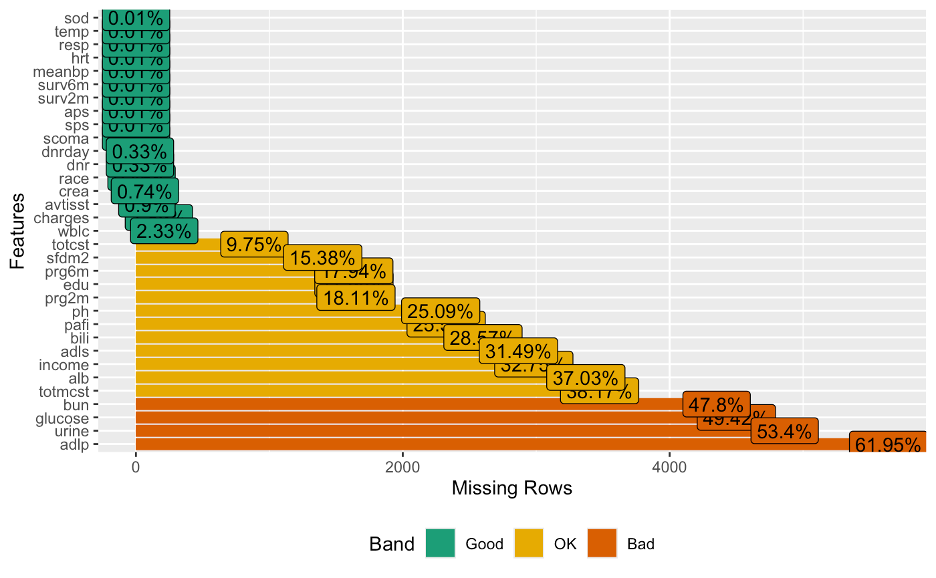
\includegraphics[width=\textwidth]{support2_missing_values}
  \caption{Distribución de valores faltantes en el dataset SUPPORT2.}
  \label{fig:support2-missing-values}
\end{figure}

\subsubsection{Distribución de nulos según mortalidad hospitalaria (hospdead)}

\begin{table}[H]
  \centering
  \caption[Nulos por variable según hospdead]{Distribución de nulos por variable según desenlace hospitalario (hospdead).}
  \label{tab:nulos-hospdead}
  \small
  \begin{tabular}{lrrrrr}
    \toprule
    \textbf{Variable} & \textbf{Nulos\_Vivos} & \textbf{Nulos\_Muertos} & \textbf{Porc\_Vivos} & \textbf{Porc\_Muertos} & \textbf{Diff} \\
    \midrule
    meanbp   &    1 &    0 &  0.01 &  0.00 &  0.01 \\
    hrt      &    1 &    0 &  0.01 &  0.00 &  0.01 \\
    resp     &    1 &    0 &  0.01 &  0.00 &  0.01 \\
    temp     &    1 &    0 &  0.01 &  0.00 &  0.01 \\
    sod      &    1 &    0 &  0.01 &  0.00 &  0.01 \\
    scoma    &    0 &    1 &  0.00 &  0.04 &  0.04 \\
    sps      &    0 &    1 &  0.00 &  0.04 &  0.04 \\
    aps      &    0 &    1 &  0.00 &  0.04 &  0.04 \\
    surv2m   &    0 &    1 &  0.00 &  0.04 &  0.04 \\
    surv6m   &    0 &    1 &  0.00 &  0.04 &  0.04 \\
    alb      & 2496 &  876 & 37.01 & 37.12 &  0.11 \\
    dnr      &   16 &   14 &  0.24 &  0.59 &  0.36 \\
    dnrday   &   16 &   14 &  0.24 &  0.59 &  0.36 \\
    crea     &   56 &   11 &  0.83 &  0.47 &  0.36 \\
    race     &   23 &   19 &  0.34 &  0.81 &  0.46 \\
    avtisst  &   75 &    7 &  1.11 &  0.30 &  0.82 \\
    charges  &  111 &   61 &  1.65 &  2.58 &  0.94 \\
    wblc     &  183 &   29 &  2.71 &  1.23 &  1.48 \\
    bun      & 3193 & 1159 & 47.34 & 49.11 &  1.77 \\
    urine    & 3569 & 1293 & 52.91 & 54.79 &  1.87 \\
    glucose  & 3298 & 1202 & 48.90 & 50.93 &  2.04 \\
    bili     & 1968 &  633 & 29.18 & 26.82 &  2.36 \\
    totcst   &  612 &  276 &  9.07 & 11.69 &  2.62 \\
    prg2m    & 1160 &  489 & 17.20 & 20.72 &  3.52 \\
    prg6m    & 1146 &  487 & 16.99 & 20.64 &  3.65 \\
    adls     & 2051 &  816 & 30.41 & 34.58 &  4.17 \\
    income   & 2087 &  895 & 30.94 & 37.92 &  6.98 \\
    totmcst  & 2432 & 1043 & 36.06 & 44.19 &  8.14 \\
    edu      & 1021 &  613 & 15.14 & 25.97 & 10.84 \\
    ph       & 1891 &  393 & 28.04 & 16.65 & 11.38 \\
    pafi     & 1927 &  398 & 28.57 & 16.86 & 11.70 \\
    sfdm2    & 1367 &   33 & 20.27 &  1.40 & 18.87 \\
    adlp     & 3476 & 2165 & 51.53 & 91.74 & 40.20 \\
    \bottomrule
  \end{tabular}
\end{table}

\subsubsection{Distribución de variables}

\paragraph{Variables continuas}

\begin{figure}[H]
  \centering
  \begin{subfigure}{0.48\textwidth}
    \centering
    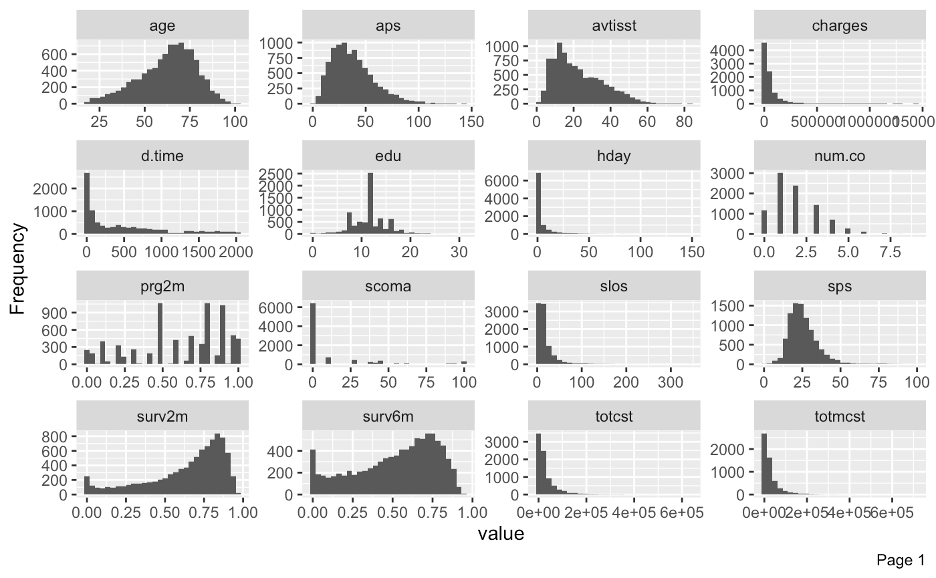
\includegraphics[width=\textwidth]{dis_continua_1}
    \caption{Distribución de variables continuas (I).}
    \label{fig:dis-continual-1}
  \end{subfigure}
  \hfill
  \begin{subfigure}{0.48\textwidth}
    \centering
    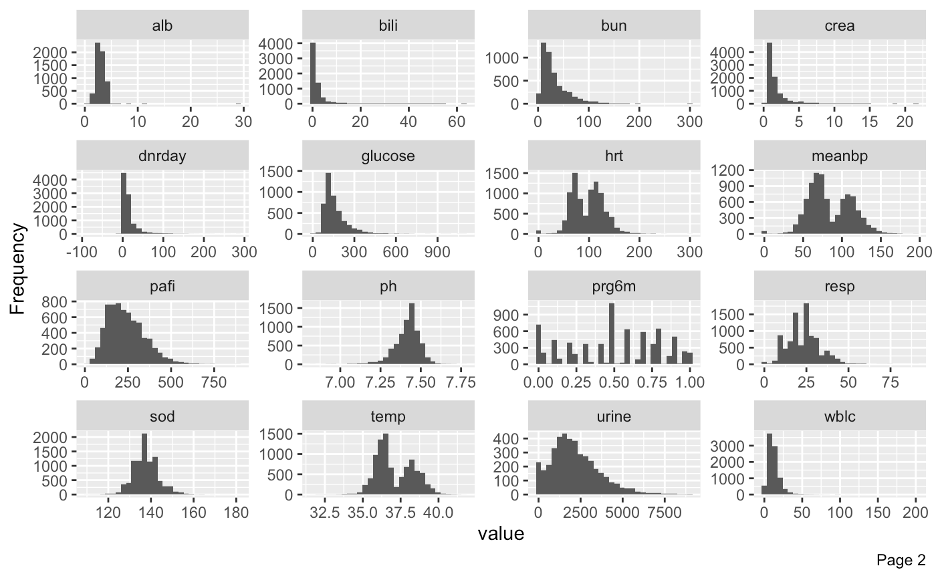
\includegraphics[width=\textwidth]{dis_continua_2}
    \caption{Distribución de variables continuas (II).}
    \label{fig:dis-continual-2}
  \end{subfigure}
  \caption{Distribución de variables continuas en SUPPORT2.}
  \label{fig:dis-continual}
\end{figure}

\paragraph{Variables categóricas}

\begin{figure}[H]
  \centering
  \begin{subfigure}{0.48\textwidth}
    \centering
    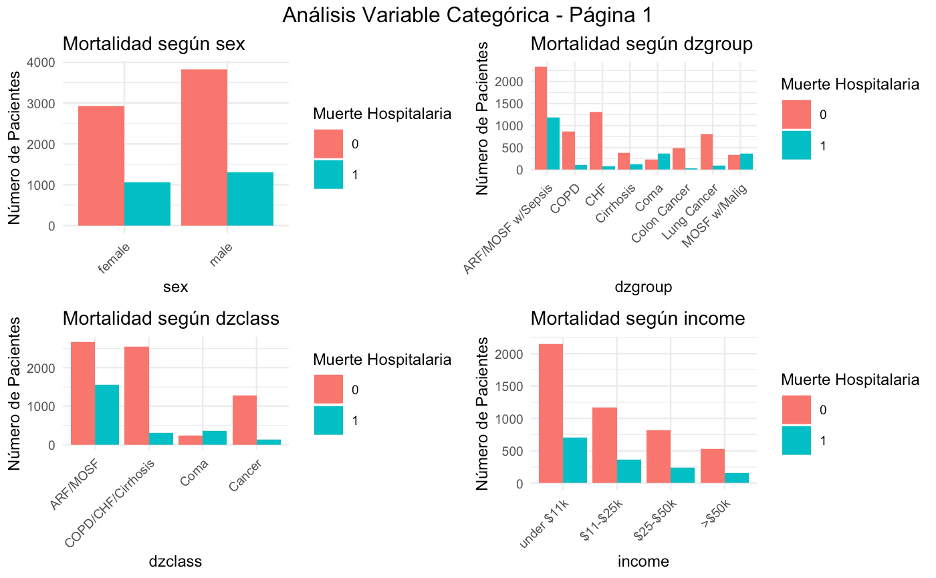
\includegraphics[width=\textwidth]{dis_categorical_1}
    \caption{Distribución de variables categóricas (I).}
    \label{fig:dis-categorical-1}
  \end{subfigure}
  \hfill
  \begin{subfigure}{0.48\textwidth}
    \centering
    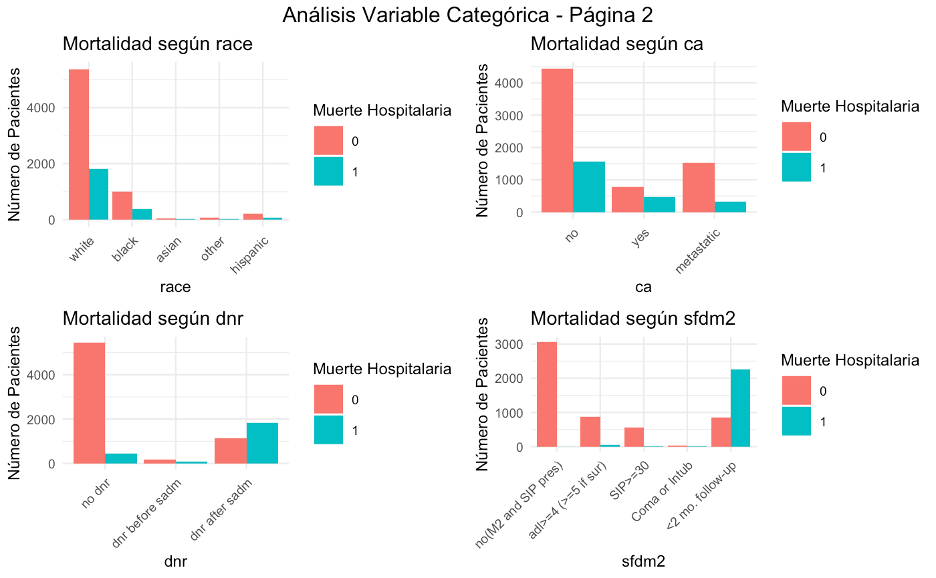
\includegraphics[width=\textwidth]{dis_categorical_2}
    \caption{Distribución de variables categóricas (II).}
    \label{fig:dis-categorical-2}
  \end{subfigure}
  \vspace{0.5em}
  \begin{subfigure}{0.48\textwidth}
    \centering
    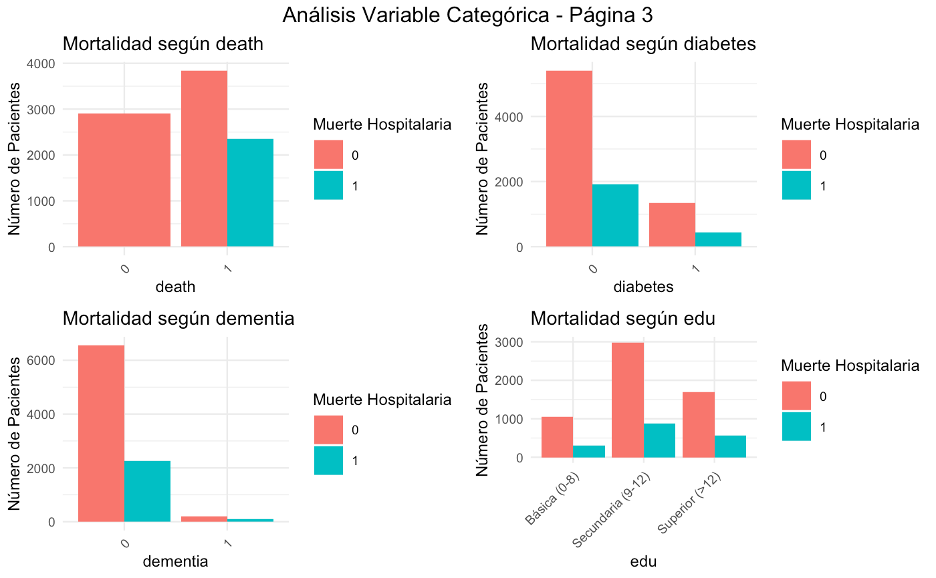
\includegraphics[width=\textwidth]{dis_categorical_3}
    \caption{Distribución de variables categóricas (III).}
    \label{fig:dis-categorical-3}
  \end{subfigure}
  \hfill
  \begin{subfigure}{0.48\textwidth}
    \centering
    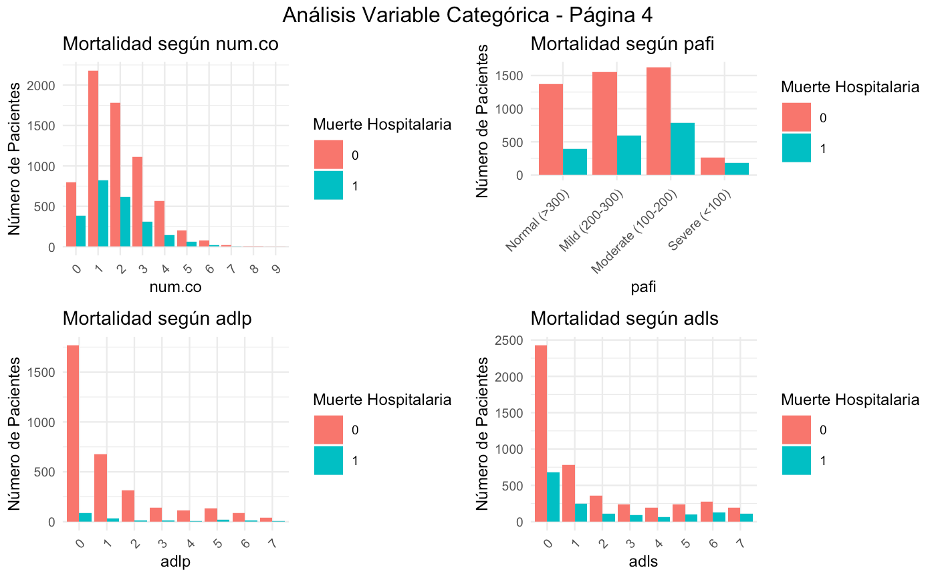
\includegraphics[width=\textwidth]{dis_categorical_4}
    \caption{Distribución de variables categóricas (IV).}
    \label{fig:dis-categorical-4}
  \end{subfigure}
  \caption{Distribución de variables categóricas en SUPPORT2.}
  \label{fig:dis-categorical}
\end{figure}

\subsubsection{Matriz de correlación}

\begin{figure}[H]
  \centering
  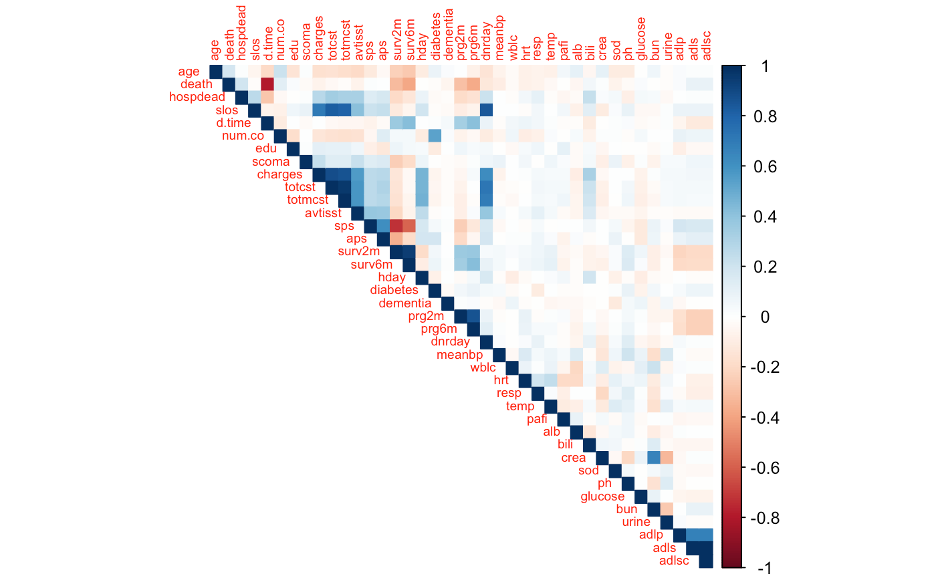
\includegraphics[width=\textwidth]{correlation_matrix}
  \caption{Matriz de correlación de variables en SUPPORT2.}
  \label{fig:correlation-matrix}
\end{figure}


\subsection{Resultados de modelos supervisados}

Los resultados del benchmarking se presentan de forma sistemática según la
estrategia de preprocesamiento (V1: Bio Data; V2: Tech Data) y el esquema de
entrenamiento utilizado (validación cruzada o entrenamiento simple sin CV). En
la nueva arquitectura experimental, los modelos se entrenaron sobre el conjunto
de entrenamiento, se compararon sobre el conjunto de validación y únicamente el
mejor modelo de cada escenario fue evaluado sobre el conjunto de prueba final.
En cada escenario se reportan las métricas AUC, sensibilidad, especificidad y
accuracy, junto con las curvas ROC comparativas de todos los modelos evaluados.

\subsubsection{V1 -- Bio Data con validación cruzada}

La Tabla~\ref{tab:v1-cv-base} resume el rendimiento de los modelos entrenados
sobre el dataset clínico-estadístico mediante validación cruzada interna y
selección posterior en el conjunto de validación. GBM obtuvo el mayor AUC
(0.947), seguido por Random Forest (0.942) y Logistic Regression (0.932).

\begin{table}[H]
  \centering
  \caption[V1 CV validación]{Rendimiento comparativo de modelos supervisados --- V1, validación cruzada, conjunto de validación (df1\_Bio).}
  \label{tab:v1-cv-base}
  \small
  \begin{tabular}{llrrrr}
    \toprule
    \textbf{Dataset} & \textbf{Modelo} & \textbf{AUC} & \textbf{Sensibilidad} & \textbf{Especificidad} & \textbf{Accuracy} \\
    \midrule
    df1\_Bio & GBM                & 0.947 & 0.749 & 0.961 & 0.906 \\
    df1\_Bio & RandomForest       & 0.942 & 0.746 & 0.948 & 0.896 \\
    df1\_Bio & LogisticRegression & 0.932 & 0.709 & 0.946 & 0.885 \\
    df1\_Bio & SVM                & 0.930 & 0.723 & 0.936 & 0.881 \\
    df1\_Bio & DecisionTree       & 0.919 & 0.698 & 0.937 & 0.875 \\
    df1\_Bio & KNN                & 0.903 & 0.573 & 0.958 & 0.858 \\
    \bottomrule
  \end{tabular}
\end{table}

La mejor configuración correspondió a GBM, con 2000 árboles, min\_n = 10,
profundidad máxima de 2, tasa de aprendizaje de 0.0068 y loss\_reduction = 0.
Al evaluar este modelo seleccionado sobre el conjunto de prueba final, se obtuvo
un AUC de 0.939, sensibilidad de 0.775, especificidad de 0.954 y accuracy de
0.906 (Tabla~\ref{tab:v1-cv-test}).

\begin{table}[H]
  \centering
  \caption[V1 CV prueba]{Evaluación final del mejor modelo --- V1, validación cruzada, conjunto de prueba.}
  \label{tab:v1-cv-test}
  \small
  \begin{tabular}{llrrrr}
    \toprule
    \textbf{Modelo} & \textbf{Dataset} & \textbf{AUC} & \textbf{Sensibilidad} & \textbf{Especificidad} & \textbf{Accuracy} \\
    \midrule
    GBM & df1\_Bio & 0.939 & 0.775 & 0.954 & 0.906 \\
    \bottomrule
  \end{tabular}
\end{table}

\begin{figure}[H]
  \centering
  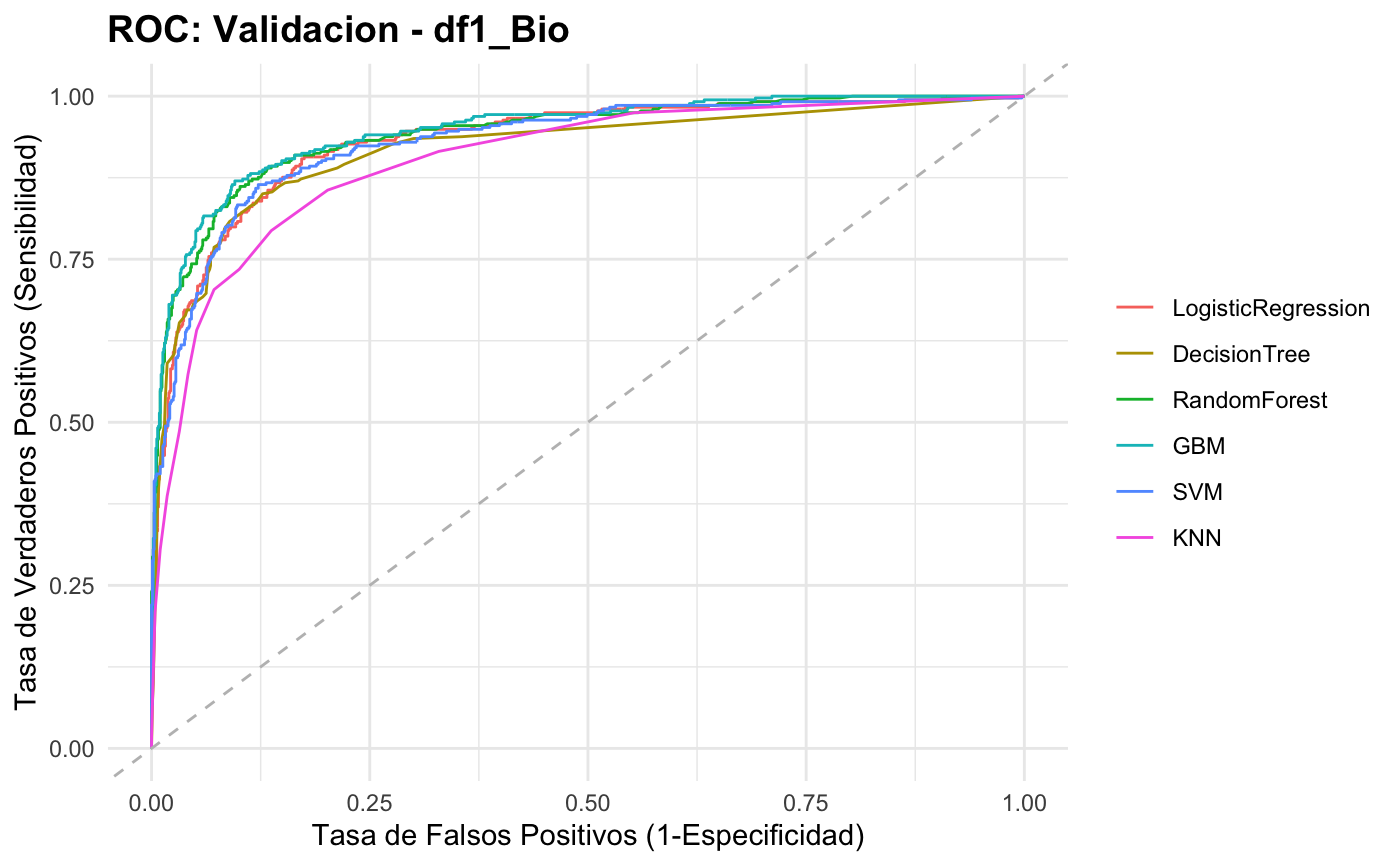
\includegraphics[width=0.85\textwidth]{bio_roc}
  \caption{Curvas ROC comparativas --- V1, validación cruzada, conjunto de validación.}
  \label{fig:roc-v1-cv}
\end{figure}

\subsubsection{V1 -- Bio Data sin validación cruzada}

La Tabla~\ref{tab:v1-nocv-base} recoge los resultados obtenidos mediante
entrenamiento simple, comparando los modelos en el conjunto de validación. GBM
alcanzó nuevamente el mayor AUC (0.949), seguido por Random Forest (0.943) y
SVM (0.934). En este escenario, Decision Tree mostró un comportamiento más
estable que en experimentos previos, con un AUC de 0.913.

\begin{table}[H]
  \centering
  \caption[V1 sin CV validación]{Rendimiento comparativo de modelos supervisados --- V1, entrenamiento simple, conjunto de validación (df1\_Bio).}
  \label{tab:v1-nocv-base}
  \small
  \begin{tabular}{llrrrr}
    \toprule
    \textbf{Dataset} & \textbf{Modelo} & \textbf{AUC} & \textbf{Sensibilidad} & \textbf{Especificidad} & \textbf{Accuracy} \\
    \midrule
    df1\_Bio & GBM                & 0.949 & 0.763 & 0.960 & 0.909 \\
    df1\_Bio & RandomForest       & 0.943 & 0.751 & 0.952 & 0.900 \\
    df1\_Bio & SVM                & 0.934 & 0.720 & 0.940 & 0.883 \\
    df1\_Bio & LogisticRegression & 0.933 & 0.701 & 0.950 & 0.885 \\
    df1\_Bio & DecisionTree       & 0.913 & 0.734 & 0.944 & 0.890 \\
    df1\_Bio & KNN                & 0.910 & 0.596 & 0.958 & 0.864 \\
    \bottomrule
  \end{tabular}
\end{table}

La mejor configuración correspondió a GBM, con 644 árboles, profundidad máxima
de 5, tasa de aprendizaje de 0.0215443, loss\_reduction = 0.0077426 y min\_n =
20. En el conjunto de prueba final, este modelo alcanzó un AUC de 0.942,
sensibilidad de 0.755, especificidad de 0.948 y accuracy de 0.896
(Tabla~\ref{tab:v1-nocv-test}).

\begin{table}[H]
  \centering
  \caption[V1 sin CV prueba]{Evaluación final del mejor modelo --- V1, entrenamiento simple, conjunto de prueba.}
  \label{tab:v1-nocv-test}
  \small
  \begin{tabular}{llrrrr}
    \toprule
    \textbf{Modelo} & \textbf{Dataset} & \textbf{AUC} & \textbf{Sensibilidad} & \textbf{Especificidad} & \textbf{Accuracy} \\
    \midrule
    GBM & df1\_Bio & 0.942 & 0.755 & 0.948 & 0.896 \\
    \bottomrule
  \end{tabular}
\end{table}

\begin{figure}[H]
  \centering
  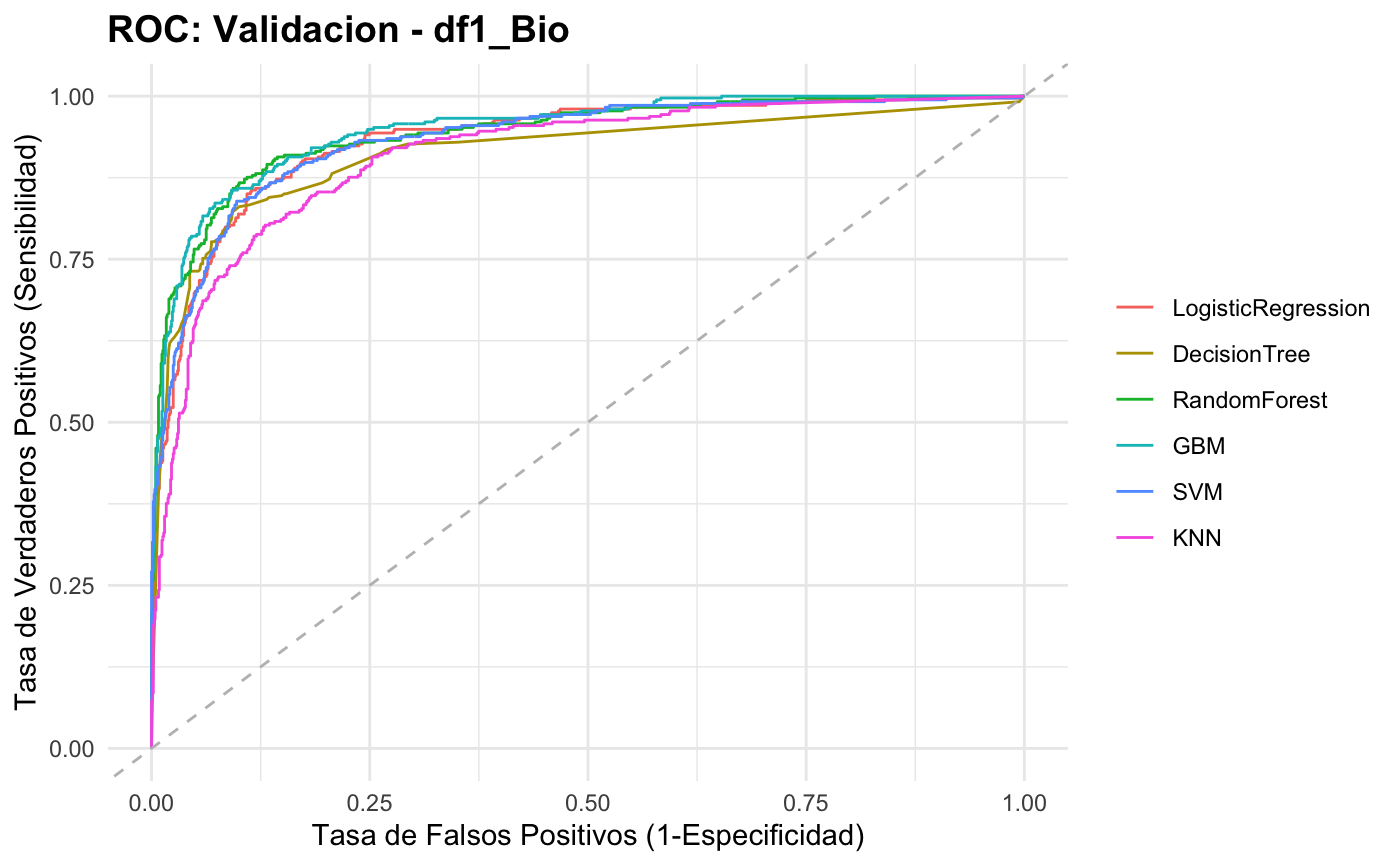
\includegraphics[width=0.85\textwidth]{bio_roc_no_cv}
  \caption{Curvas ROC comparativas --- V1, entrenamiento simple, conjunto de validación.}
  \label{fig:roc-v1-nocv}
\end{figure}

\subsubsection{V2 -- Tech Data con validación cruzada}

La Tabla~\ref{tab:v2-cv-base} presenta los resultados sobre el dataset
técnico-estadístico mediante validación cruzada interna y selección en el
conjunto de validación. Random Forest y GBM alcanzaron el AUC más alto (0.978),
seguidos por SVM (0.973) y Logistic Regression (0.972), superando claramente a
los modelos de la estrategia V1 en este escenario.

\begin{table}[H]
  \centering
  \caption[V2 CV validación]{Rendimiento comparativo de modelos supervisados --- V2, validación cruzada, conjunto de validación (df2\_Tech).}
  \label{tab:v2-cv-base}
  \small
  \begin{tabular}{llrrrr}
    \toprule
    \textbf{Dataset} & \textbf{Modelo} & \textbf{AUC} & \textbf{Sensibilidad} & \textbf{Especificidad} & \textbf{Accuracy} \\
    \midrule
    df2\_Tech & RandomForest       & 0.978 & 0.824 & 0.955 & 0.921 \\
    df2\_Tech & GBM                & 0.978 & 0.815 & 0.957 & 0.920 \\
    df2\_Tech & SVM                & 0.973 & 0.827 & 0.956 & 0.922 \\
    df2\_Tech & LogisticRegression & 0.972 & 0.824 & 0.956 & 0.921 \\
    df2\_Tech & DecisionTree       & 0.966 & 0.812 & 0.945 & 0.910 \\
    df2\_Tech & KNN                & 0.958 & 0.736 & 0.952 & 0.895 \\
    \bottomrule
  \end{tabular}
\end{table}

La mejor configuración correspondió a Random Forest, con mtry = 15 y min\_n =
2. En la evaluación final sobre el conjunto de prueba, este modelo obtuvo un AUC
de 0.974, sensibilidad de 0.849, especificidad de 0.957 y accuracy de 0.928
(Tabla~\ref{tab:v2-cv-test}).

\begin{table}[H]
  \centering
  \caption[V2 CV prueba]{Evaluación final del mejor modelo --- V2, validación cruzada, conjunto de prueba.}
  \label{tab:v2-cv-test}
  \small
  \begin{tabular}{llrrrr}
    \toprule
    \textbf{Modelo} & \textbf{Dataset} & \textbf{AUC} & \textbf{Sensibilidad} & \textbf{Especificidad} & \textbf{Accuracy} \\
    \midrule
    RandomForest & df2\_Tech & 0.974 & 0.849 & 0.957 & 0.928 \\
    \bottomrule
  \end{tabular}
\end{table}

\begin{figure}[H]
  \centering
  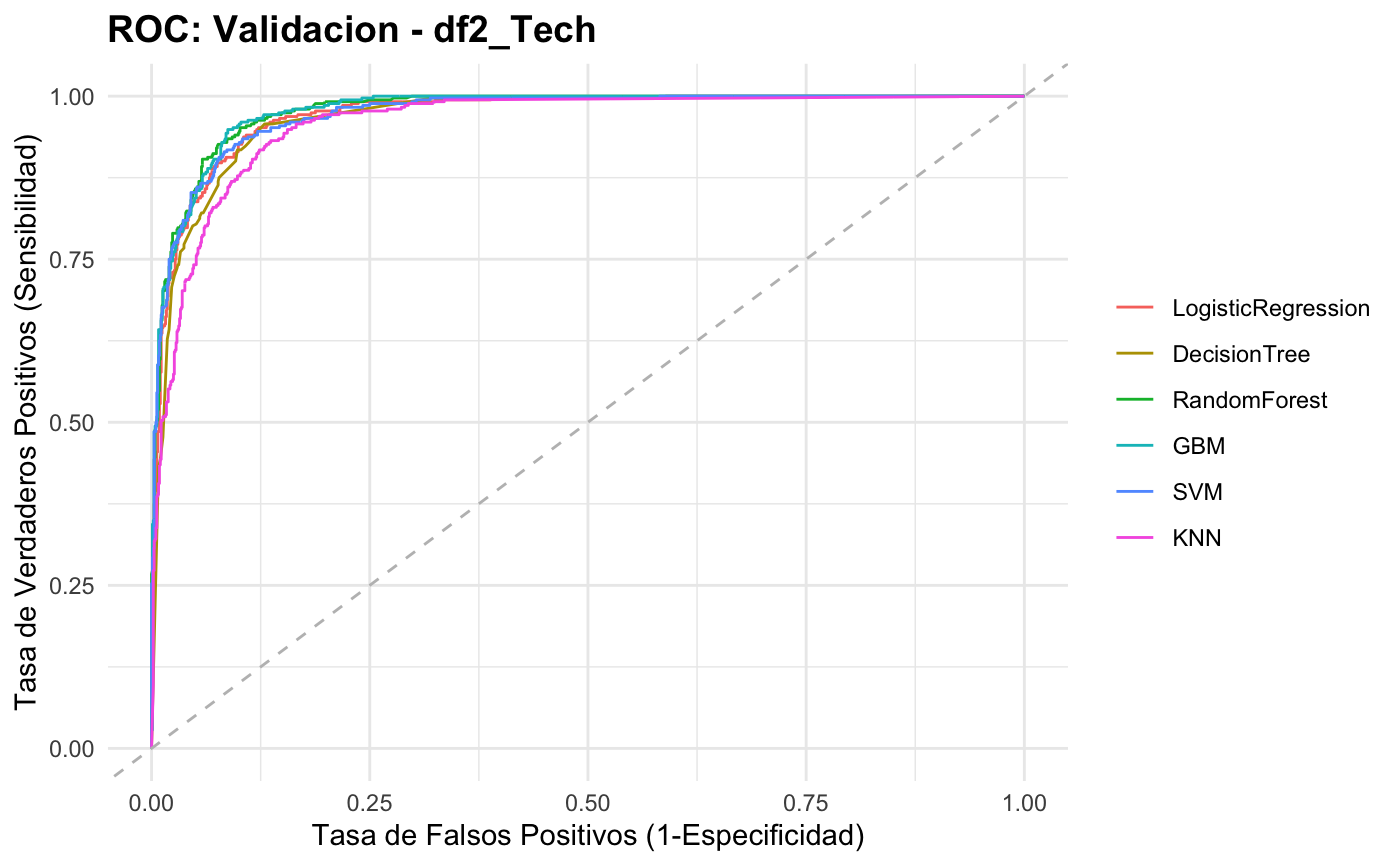
\includegraphics[width=0.85\textwidth]{tech_roc}
  \caption{Curvas ROC comparativas --- V2, validación cruzada, conjunto de validación.}
  \label{fig:roc-v2-cv}
\end{figure}

\subsubsection{V2 -- Tech Data sin validación cruzada}

La Tabla~\ref{tab:v2-nocv-base} muestra los resultados con entrenamiento simple
y comparación en el conjunto de validación. GBM obtuvo el mayor AUC (0.978),
seguido muy de cerca por Random Forest (0.977), SVM (0.973) y Logistic
Regression (0.973). La proximidad entre los modelos principales sugiere una alta
capacidad predictiva de la representación técnico-estadística del dataset.

\begin{table}[H]
  \centering
  \caption[V2 sin CV validación]{Rendimiento comparativo de modelos supervisados --- V2, entrenamiento simple, conjunto de validación (df2\_Tech).}
  \label{tab:v2-nocv-base}
  \small
  \begin{tabular}{llrrrr}
    \toprule
    \textbf{Dataset} & \textbf{Modelo} & \textbf{AUC} & \textbf{Sensibilidad} & \textbf{Especificidad} & \textbf{Accuracy} \\
    \midrule
    df2\_Tech & GBM                & 0.978 & 0.821 & 0.955 & 0.920 \\
    df2\_Tech & RandomForest       & 0.977 & 0.832 & 0.957 & 0.924 \\
    df2\_Tech & SVM                & 0.973 & 0.830 & 0.957 & 0.924 \\
    df2\_Tech & LogisticRegression & 0.973 & 0.838 & 0.953 & 0.923 \\
    df2\_Tech & DecisionTree       & 0.966 & 0.790 & 0.944 & 0.904 \\
    df2\_Tech & KNN                & 0.962 & 0.741 & 0.954 & 0.898 \\
    \bottomrule
  \end{tabular}
\end{table}

La mejor configuración correspondió a GBM, con 200 árboles, profundidad máxima
de 6, tasa de aprendizaje de 0.0464159, loss\_reduction = 0.0464159 y min\_n =
12. En el conjunto de prueba final, este modelo alcanzó un AUC de 0.975,
sensibilidad de 0.841, especificidad de 0.950 y accuracy de 0.920
(Tabla~\ref{tab:v2-nocv-test}).

\begin{table}[H]
  \centering
  \caption[V2 sin CV prueba]{Evaluación final del mejor modelo --- V2, entrenamiento simple, conjunto de prueba.}
  \label{tab:v2-nocv-test}
  \small
  \begin{tabular}{llrrrr}
    \toprule
    \textbf{Modelo} & \textbf{Dataset} & \textbf{AUC} & \textbf{Sensibilidad} & \textbf{Especificidad} & \textbf{Accuracy} \\
    \midrule
    GBM & df2\_Tech & 0.975 & 0.841 & 0.950 & 0.920 \\
    \bottomrule
  \end{tabular}
\end{table}

\begin{figure}[H]
  \centering
  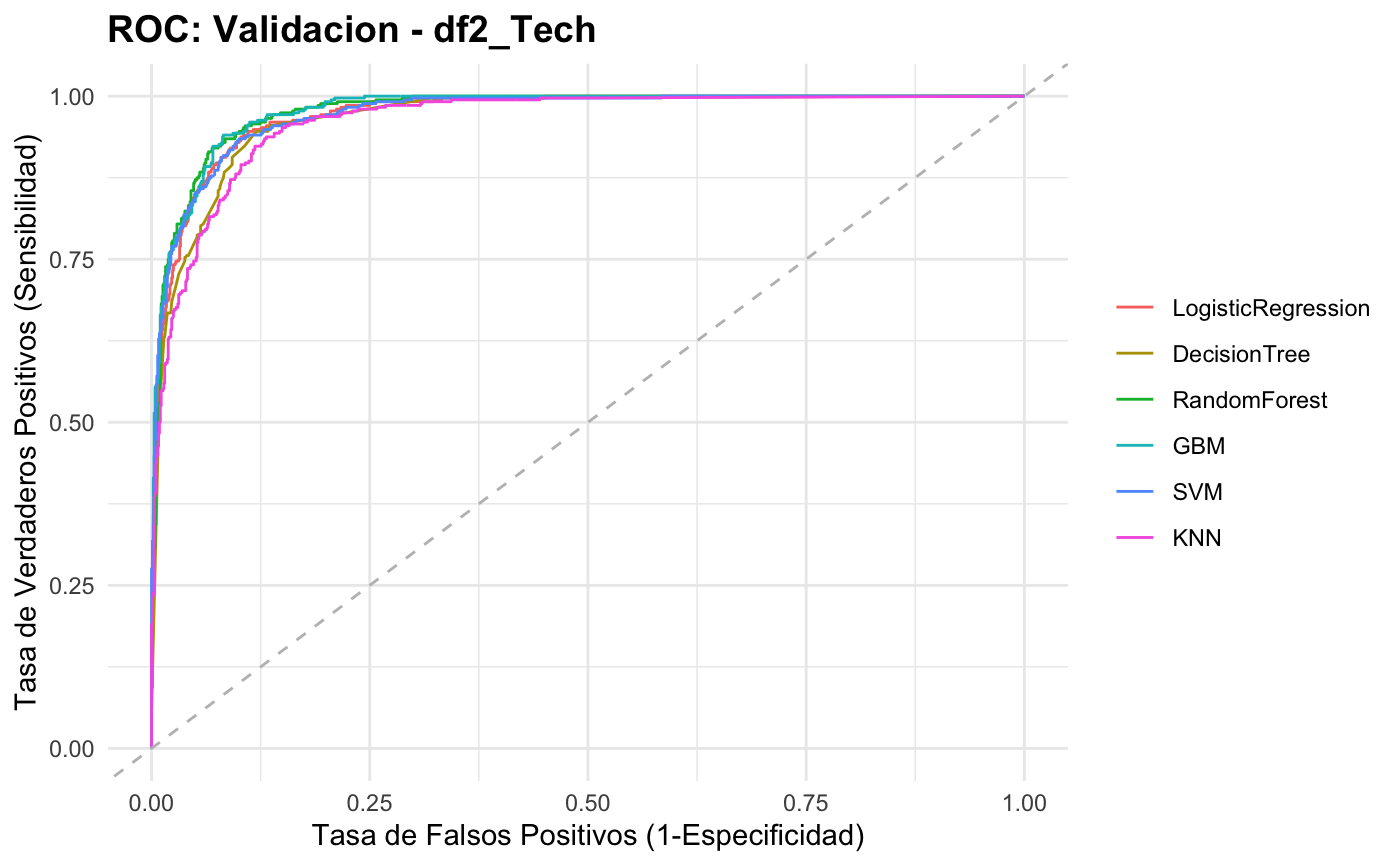
\includegraphics[width=0.85\textwidth]{tech_roc_no_cv}
  \caption{Curvas ROC comparativas --- V2, entrenamiento simple, conjunto de validación.}
  \label{fig:roc-v2-nocv}
\end{figure}

\section{Discusión}\label{sec:discusion}

\subsection{Comparación entre estrategias de preprocesamiento}

Desde un punto de vista estrictamente numérico, la estrategia
técnico-estadística (V2) obtuvo métricas superiores. Mientras que en la
estrategia clínico-estadística (V1) los mejores modelos, Random Forest y GBM,
alcanzaron valores de AUC próximos a 0.947--0.949 en validación y 0.939--0.942
en prueba, en la V2 estos mismos modelos alcanzaron valores cercanos a 0.978 en
validación y 0.974--0.975 en prueba.

Sin embargo, en medicina predictiva, el mayor rendimiento métrico no implica
necesariamente una mayor validez clínica. La diferencia observada en AUC sugiere
que la estrategia V2 podría beneficiarse de variables que la estrategia V1
excluyó por riesgo de \textit{Data Leakage} o por menor coherencia biológica. En
este sentido, la V2 ofrece mayor rendimiento estadístico, mientras que la V1
representa una aproximación más prudente desde el punto de vista clínico y
metodológico.

\subsection{Contraste de la hipótesis}

La hipótesis planteada proponía que el preprocesamiento con criterio clínico
mejoraría la calidad del modelo. Los resultados muestran una confirmación
parcial:

\begin{itemize}
  \item En términos de estabilidad, la estrategia V1 mantiene resultados muy
    consistentes entre la versión con CV y sin CV para los modelos de ensamble.
  \item En términos de rendimiento bruto, la V2 supera a la V1.
  \item En términos de evaluación final, el conjunto de prueba confirma la misma
    tendencia observada durante la validación, sin alterar la selección del mejor
    modelo.
\end{itemize}

Esta diferencia refuerza la necesidad de interpretar el rendimiento predictivo
junto con la procedencia y disponibilidad real de las variables. La V2
probablemente retuvo información que facilita la predicción estadística, pero
que en un entorno hospitalario real al momento del ingreso podría no estar
disponible o presentar riesgo de contaminación temporal. La V1, aunque no
maximiza el AUC, mantiene un rendimiento elevado (AUC > 0.93 en prueba) bajo un
criterio de mayor fidelidad clínica.

\subsection{Impacto del conocimiento clínico}

El impacto del conocimiento clínico se observa en la curación del conjunto de
datos:

\begin{enumerate}
  \item Imputación estratificada: Aunque la V1 utiliza un conjunto más restringido
    de variables predictoras, la combinación de imputaciones contextualizadas y
    eliminaciones estratégicas permitió que modelos como Random Forest
    y GBM alcanzaran AUC superiores a 0.94 en validación. Esto sugiere que los
    predictores conservados mantienen una alta capacidad informativa.
  \item Sensibilidad y especificidad: En V1, la especificidad se mantiene en
    valores elevados (aprox. 0.93--0.95). Este comportamiento indica una buena
    capacidad para identificar correctamente a los pacientes supervivientes, un
    aspecto relevante para reducir falsas alarmas en contextos de asignación de
    recursos críticos.
  \item Rendimiento de KNN: Las Tablas~\ref{tab:v1-cv-base},
    \ref{tab:v1-nocv-base}, \ref{tab:v2-cv-base} y
    \ref{tab:v2-nocv-base} muestran que KNN fue superado por los métodos
    basados en árboles, aun cuando la normalización fue integrada dentro del
    flujo de tidymodels. Esto valida que la relación entre las variables
    clínicas y la mortalidad no es necesariamente lineal ni depende solo de
    distancias simples.
\end{enumerate}

\subsection{Comportamiento de los modelos}

\begin{itemize}
  \item Modelos de ensamble: Random Forest (RF) y Stochastic Gradient Boosting
    (GBM) mostraron el mejor rendimiento global. GBM lideró los escenarios V1,
    mientras que Random Forest y GBM presentaron rendimientos prácticamente
    equivalentes en V2. Este patrón refleja su capacidad para capturar
    interacciones no lineales entre variables clínicas.
  \item Regresión logística: Este modelo alcanzó AUC superiores a 0.93 en Bio Data,
    lo que sugiere que varias de las variables clínicas seleccionadas mantienen
    una relación discriminativa estable con la mortalidad. Además, su mayor
    interpretabilidad la convierte en una referencia útil frente a modelos más
    complejos.
  \item Support Vector Machine: La incorporación de SVM permitió evaluar un modelo
    de margen máximo plenamente integrado en el flujo tidymodels. Su rendimiento
    fue competitivo, especialmente en V2, aunque no superó de forma consistente
    a los modelos de ensamble.
  \item Decision Tree (rpart): A diferencia de experimentos previos, el árbol de
    decisión simple mantuvo un rendimiento discriminativo razonable en los
    escenarios actualizados. Sin embargo, continuó por debajo de Random Forest y
    GBM, lo que subraya la ventaja de los métodos de ensamble en problemas
    biomédicos con relaciones no lineales y variables heterogéneas.
\end{itemize}

\section{Conclusiones}\label{sec:conclusiones}

La ejecución de esta investigación permite concluir que la robustez de un sistema
predictivo en salud depende tanto de la capacidad de los algoritmos como de la
calidad metodológica del flujo de preprocesamiento. Mediante un esquema modular
y reproducible, se observó que los modelos de ensamble, específicamente Random
Forest y Gradient Boosting Machine (GBM), lideraron la capacidad de
discriminación con valores de AUC de hasta 0.949 en validación y 0.942 en prueba
en el escenario clínico-estadístico, y de hasta 0.978 en validación y 0.975 en
prueba en el escenario técnico-estadístico. Estos resultados indican
que, ante variables fisiológicas con alta variabilidad, multicolinealidad y
relaciones no lineales, los algoritmos basados en árboles presentan ventajas
frente a aproximaciones lineales, de margen o basadas en distancia como SVM y
KNN. La regresión logística también mostró un rendimiento relevante, con AUC
superiores a 0.93 en el escenario biológico, lo que sugiere que parte de los
predictores seleccionados mantienen una relación discriminativa estable con la
mortalidad hospitalaria. La evaluación final sobre el conjunto de prueba,
reservada únicamente para el mejor modelo de cada escenario, permitió confirmar
la tendencia observada en validación sin utilizar el test como criterio de
selección.

El aporte principal de este trabajo reside en mostrar que el preprocesamiento
informado por conocimiento clínico no debe evaluarse únicamente por la
optimización métrica, sino también por su capacidad para preservar la validez
metodológica del experimento. La comparación entre la estrategia basada en
lógica clínica y la estrategia técnica reveló una paradoja relevante: aunque los
métodos automatizados pueden alcanzar valores superiores de AUC, dichos
resultados pueden estar influidos por la retención de variables con potenciales
sesgos o riesgo de \textit{Data Leakage}. La eliminación de variables de
seguimiento temporal y de estimaciones derivadas de modelos previos, junto con
la imputación estratificada por grupo diagnóstico, permitió preservar mejor la
coherencia biológica del conjunto de datos. Además, el análisis del carácter
informativo de los valores faltantes en las escalas de dependencia funcional
mostró que la ausencia de datos no siempre representa un error técnico, sino que
puede constituir una señal clínica relevante. Como limitación principal, la
validez de estos hallazgos se encuentra acotada a la cohorte SUPPORT2 y debe ser
interpretada con cautela fuera de este contexto. En conjunto, el estudio
respalda la integración del razonamiento clínico en el preprocesamiento como una
condición necesaria para desarrollar modelos predictivos no solo precisos, sino
también metodológicamente defendibles.


% --- Declaración de uso de IA -----------------------------------------------
\newpage
\phantomsection
\addcontentsline{toc}{section}{Declaración de uso de inteligencia artificial}
\noindent\textbf{Declaración de uso de inteligencia artificial}

Durante la elaboración de este Trabajo Fin de Máster se emplearon herramientas
de inteligencia artificial generativa como apoyo en la redacción, la
organización del proceso documentado y la búsqueda y síntesis preliminar de
información, incluyendo Codex, Cursor, Gemini, ChatGPT y Google AI Studio. Su
uso fue complementario y no sustituyó el criterio del autor. Todas las
decisiones metodológicas fueron tomadas por el autor en coordinación con las
orientaciones del asesor.

% --- Bibliografía ------------------------------------------------------------
\newpage
\bibliography{references}

% --- Anexos -----------------------------------------------------------------
\newpage
\section{Anexos}\label{sec:anexos}

\subsection{Estructura de carpetas del proyecto}\label{sec:anexo-estructura}

\begin{lstlisting}[basicstyle=\small\ttfamily]
TFM-ML-Benchmark/
|-- data/
|   |-- raw/
|   `-- processed/support2/
|       |-- df1/  # estrategia clinico-estadistica
|       `-- df2/  # estrategia tecnico-estadistica
|-- eda/
|-- preprocessing/
|-- models/
|-- scripts/modeling_utils_tidymodels_clean.R
|-- figures/
`-- manuscript/
\end{lstlisting}

\subsection{Diccionario de variables del dataset SUPPORT2}\label{sec:anexo-diccionario}

\begingroup
\small
\setlength{\tabcolsep}{4pt}
\begin{longtable}{p{2.1cm}p{1.4cm}p{6.7cm}p{3.8cm}}
\caption{Diccionario de variables del dataset SUPPORT2.}\label{tab:diccionario-support2}\\
\toprule
\textbf{Variable} & \textbf{Tipo} & \textbf{Descripción} & \textbf{Unidades / Valores posibles} \\
\midrule
\endfirsthead
\toprule
\textbf{Variable} & \textbf{Tipo} & \textbf{Descripción} & \textbf{Unidades / Valores posibles} \\
\midrule
\endhead
id & Entero & Identificador único del paciente en el estudio. & Número único \\
age & Continuo & Edad del paciente al ingresar al estudio. & Años \\
death & Continuo & Fallecimiento en cualquier momento del seguimiento (hasta el 31/DIC/1994). & 0 = No, 1 = Sí \\
sex & Categórico & Género biológico del paciente. & male (hombre), female (mujer) \\
hospdead & Binario & Fallecimiento ocurrido dentro del hospital durante el ingreso. & 0 = No, 1 = Sí \\
slos & Continuo & Días transcurridos desde el ingreso al estudio hasta el alta. & Días \\
d.time & Continuo & Días totales de seguimiento del paciente en el estudio. & Días \\
dzgroup & Categórico & Subcategoría específica del diagnóstico principal de ingreso. & ARF/MOSF con Sepsis, CHF, COPD, Cirrosis, Cáncer de Colon, Coma, Cáncer de Pulmón, MOSF con Malignidad \\
dzclass & Categórico & Categoría general de la enfermedad (agrupación de dzgroup). & ``ARF/MOSF'', ``COPD/CHF/Cirrhosis'', ``Cancer'', ``Coma'' \\
num.co & Continuo & Número de comorbilidades (enfermedades simultáneas). A mayor valor, peor pronóstico. & Número ordinal \\
edu & Categórico & Nivel educativo medido en años de escolaridad. & Años \\
income & Categórico & Nivel estimado de ingresos económicos anuales del paciente. & ``under \$11k'', ``\$11-\$25k'', ``\$25-\$50k'', ``>\$50k'' \\
scoma & Continuo & Puntuación de coma basada en la escala de Glasgow en el día 3 (predicha por modelo). & Escala numérica \\
charges & Continuo & Cargos o costos económicos facturados por el hospital. & Dólares (\$) \\
totcst & Continuo & Costo total calculado mediante la relación costo-cargo (RCC). & Dólares (\$) \\
totmcst & Continuo & Micro-costo total calculado para el paciente. & Dólares (\$) \\
avtisst & Continuo & Puntuación promedio TISS (días 3-25). Mide la intensidad de intervenciones terapéuticas en UCI. & Escala TISS \\
race & Categórico & Etnia o raza registrada del paciente. & asian, black, hispanic, missing, other, white \\
sps & Continuo & Puntuación de fisiología SUPPORT en el día 3 (predicha por modelo). & Escala numérica \\
aps & Continuo & Puntuación fisiológica APACHE III en el día 3 (sin coma, con BUN corregido y diuresis). & Escala numérica \\
surv2m & Continuo & Estimación del modelo SUPPORT de la probabilidad de supervivencia a los 2 meses (en el día 3). & Probabilidad (0 a 1) \\
surv6m & Continuo & Estimación del modelo SUPPORT de la probabilidad de supervivencia a los 6 meses (en el día 3). & Probabilidad (0 a 1) \\
hday & Entero & Día de hospitalización en el que el paciente ingresó formalmente al estudio. & Días \\
diabetes & Continuo & Presencia de diabetes mellitus como enfermedad comórbida preexistente. & 0 = No, 1 = Sí \\
dementia & Continuo & Presencia de demencia crónica como enfermedad comórbida preexistente. & 0 = No, 1 = Sí \\
ca & Categórico & Estado de enfermedad oncológica activa en el paciente. & no (sano), yes (cáncer localizado), metastatic (metástasis) \\
prg2m & Continuo & Estimación subjetiva del médico sobre la probabilidad de supervivencia a 2 meses. & Probabilidad (0 a 1) \\
prg6m & Categórico & Estimación subjetiva del médico sobre la probabilidad de supervivencia a 6 meses. & Probabilidad (0 a 1) \\
dnr & Categórico & Estado de la orden de No Reanimación (DNR) y el momento de su firma. & no dnr, dnr before sadm, dnr after sadm, missing \\
dnrday & Continuo & Día del ingreso en que se firmó la orden DNR (valores negativos indican pre-ingreso). & Días \\
meanbp & Continuo & Presión arterial media (PAM) del paciente registrada en el día 3. & mmHg \\
wblc & Continuo & Conteo total de glóbulos blancos en sangre en el día 3. & Miles por $\mu$L \\
hrt & Continuo & Frecuencia cardíaca registrada en el día 3. & Latidos por minuto (lpm) \\
resp & Continuo & Frecuencia respiratoria registrada en el día 3. & Respiraciones por minuto (rpm) \\
temp & Continuo & Temperatura corporal medida en el día 3. & Grados Celsius (°C) \\
pafi & Continuo & Índice de oxigenación Kirby ($PaO_2/FiO_2$). Indicador clínico clave de hipoxemia. & Ratio (mmHg) \\
alb & Continuo & Nivel de albúmina sérica (proteína) medido en el día 3. & g/dL \\
bili & Continuo & Nivel de bilirrubina total en sangre medido en el día 3. & mg/dL \\
crea & Continuo & Nivel de creatinina sérica en sangre (función renal) medido en el día 3. & mg/dL \\
sod & Continuo & Concentración de sodio sérico en sangre medida en el día 3. & mEq/L \\
ph & Continuo & pH de la sangre arterial medido en el día 3 (equilibrio ácido-base). & Escala de pH (6.8 a 7.8) \\
glucose & Entero & Nivel de glucosa en sangre medido en el día 3. & mg/dL \\
bun & Entero & Nitrógeno ureico en sangre (función renal/metabólica) medido en el día 3. & mg/dL \\
urine & Entero & Gasto urinario (diuresis total de 24 horas) medido en el día 3. & mL \\
adlp & Categórico & Índice de Actividades de la Vida Diaria (ADL) respondido por el propio paciente. & Escala ordinal \\
adls & Continuo & Índice de Actividades de la Vida Diaria (ADL) respondido por un familiar/representante. & Escala ordinal \\
sfdm2 & Categórico & Escala de discapacidad funcional (SIP) a los 2 meses. El nivel 5 denota muerte temprana. & Escala 1 al 5 \\
adlsc & Continuo & Índice ADL imputado y calibrado estadísticamente con respecto al reporte del familiar. & Escala numérica \\
\bottomrule
\end{longtable}
\endgroup

 
\end{document}
